% =====================================================================
%  Exposé gRPC — Master 1 Web Services — UASZ
%  Medoune MASSALY & Alioune DIOUF — 9 décembre 2026
%  Compilation : latexmk -pdf expose-grpc.tex   (ou pdflatex deux fois)
% =====================================================================
\documentclass[aspectratio=169,11pt]{beamer}
\usepackage[french]{babel}
\frenchsetup{StandardLists=true}
\usetheme{grpc}
\usepackage{pgfplots}
\pgfplotsset{compat=1.18}
\usepackage{qrcode}

\DeclareUnicodeCharacter{2192}{\ensuremath{\rightarrow}}
\DeclareUnicodeCharacter{2190}{\ensuremath{\leftarrow}}
\DeclareUnicodeCharacter{2264}{\ensuremath{\leq}}
\DeclareUnicodeCharacter{2265}{\ensuremath{\geq}}
\DeclareUnicodeCharacter{2248}{\ensuremath{\approx}}
\DeclareUnicodeCharacter{2212}{\ensuremath{-}}
\DeclareUnicodeCharacter{00D7}{\ensuremath{\times}}

\title{gRPC}
\subtitle{Des appels de procédure à distance modernes}
\author{Medoune MASSALY \& Alioune DIOUF}
\date{9 décembre 2026}
\institute{Université Assane Seck de Ziguinchor}

% Étape numérotée (pastille ambre)
\newcommand{\etape}[1]{\tikz[baseline=(e.base)]\node[circle,fill=Amber,text=white,inner sep=1pt,
  minimum size=1.25em,font=\scriptsize\bfseries](e){#1};}
% Légende qui change à chaque étape d'une animation (la dernière reste dans le polycopié)
\newcommand{\legendefin}[2]{\only<#1>{\etape{#1}\enspace #2}}
\newcommand{\legende}[2]{\only<#1| handout:0>{\etape{#1}\enspace #2}}

% Pages de section : fond nuit, grand numéro, sommaire à droite
\AtBeginSection[]{%
  \begin{frame}[plain,noframenumbering]
    \begin{tikzpicture}[remember picture,overlay]
      \fill[Navy] (current page.south west) rectangle (current page.north east);
      \draw[step=0.5cm,white,opacity=0.04] (current page.south west) grid (current page.north east);
      \node[hexa=5.2cm,draw=Teal,line width=1pt,opacity=0.3] at ([xshift=-1.3cm,yshift=1.1cm]current page.south east) {};
      \node[hexa=3.2cm,draw=TealGlow,line width=0.6pt,opacity=0.2] at ([xshift=-3.5cm,yshift=0.5cm]current page.south east) {};
      \node[anchor=north west,font=\ttfamily\bfseries,text=TealGlow,scale=3.6]
        at ([xshift=0.9cm,yshift=-1.0cm]current page.north west) {0\insertsectionnumber};
      \node[anchor=north west,text=white,font=\huge\bfseries,text width=8cm,align=left]
        at ([xshift=0.9cm,yshift=-3.3cm]current page.north west) {\insertsectionhead};
      \foreach \n/\nom in {1/Introduction, 2/Fonctionnement, 3/{Langage de définition (IDL)},
          4/{Avantages et inconvénients}, 5/Sécurité, 6/{Tableau comparatif}, 7/{TP et démonstration}, 8/Conclusion} {
        \ifnum\n=\value{section}
          \fill[TealGlow] ([xshift=-6.05cm,yshift={-0.75cm-\n*0.56cm+0.2cm}]current page.north east) rectangle ++(0.07,-0.4);
          \node[anchor=west,font=\small\bfseries,text=white]
            at ([xshift=-5.8cm,yshift={-0.75cm-\n*0.56cm}]current page.north east) {{\color{TealGlow}\ttfamily 0\n}\enspace\nom};
        \else
          \node[anchor=west,font=\small,text=CodeMuted]
            at ([xshift=-5.8cm,yshift={-0.75cm-\n*0.56cm}]current page.north east) {{\ttfamily 0\n}\enspace\nom};
        \fi
      }
    \end{tikzpicture}
  \end{frame}
}

\begin{document}
% Les raccourcis français (; : ! ? actifs) cassent TikZ dans les diapos Beamer
\shorthandoff{;:!?}

% =====================================================================
%  PAGE DE TITRE
% =====================================================================
\begin{frame}[plain,noframenumbering]
  \begin{tikzpicture}[remember picture,overlay]
    \fill[Navy] (current page.south west) rectangle (current page.north east);
    \draw[step=0.5cm,white,opacity=0.04] (current page.south west) grid (current page.north east);
    \begin{scope}[shift={([xshift=-3.5cm,yshift=0.2cm]current page.east)}]
      \foreach \x/\y/\o in {0/0/1, 1.73/1/0.35, 1.73/-1/0.35, -1.73/1/0.2, 0/2/0.25, 0/-2/0.25, -1.73/-1/0.15}
        \node[hexa=1.95cm,draw=Teal,line width=0.9pt,opacity=\o] at (\x,\y) {};
      \node[hexa=1.95cm,fill=Teal] at (0,0) {};
      \node[font=\ttfamily\bfseries\Huge,text=white] at (0,-0.05) {g};
      \foreach \a in {30,150,270} {
        \draw[TealGlow,line width=0.8pt,dash pattern=on 3pt off 2pt,opacity=0.7] (\a:1.1) -- (\a:3.2);
        \node[circle,fill=AmberLight,inner sep=2pt] at (\a:2.4) {};
      }
    \end{scope}
    \node[anchor=north west,font=\ttfamily\scriptsize,text=TealGlow]
      at ([xshift=1cm,yshift=-1.05cm]current page.north west) {EXPOSÉ \textperiodcentered{} WEB SERVICES \textperiodcentered{} MASTER 1};
    \node[anchor=north west,text=white,font=\fontsize{58}{58}\selectfont\bfseries]
      at ([xshift=0.92cm,yshift=-1.55cm]current page.north west) {gRPC};
    \node[anchor=north west,text=white,text width=9.2cm,font=\large,align=left]
      at ([xshift=1cm,yshift=-3.55cm]current page.north west)
      {Des appels de procédure à distance modernes~: {\color{TealGlow}HTTP/2}, {\color{TealGlow}Protocol Buffers} et {\color{AmberLight}streaming}};
    \node[anchor=south west,text=white,font=\normalsize\bfseries]
      at ([xshift=1cm,yshift=1.45cm]current page.south west) {Medoune MASSALY \enspace\&\enspace Alioune DIOUF};
    \node[anchor=south west,text=CodeMuted,font=\footnotesize]
      at ([xshift=1cm,yshift=0.85cm]current page.south west) {Université Assane Seck de Ziguinchor \textperiodcentered{} 9 décembre 2026};
  \end{tikzpicture}
\end{frame}

% =====================================================================
%  PLAN
% =====================================================================
\begin{frame}{Plan de l'exposé}
  \vspace{0.2cm}
  \centering
  \begin{tikzpicture}[
      item/.style={box,minimum width=4.35cm,minimum height=1.55cm,align=left,text width=3.95cm,anchor=north west}]
    \foreach \i/\t/\d [count=\k from 0] in {
      1/Introduction/{Qu'est-ce que gRPC, d'où vient-il~?},
      2/Fonctionnement/{HTTP/2, Protobuf, requêtes et réponses},
      3/Langage de définition/{Le fichier \mono{.proto} (IDL)},
      4/Avantages et inconvénients/{Forces, limites, gRPC-Web},
      5/Sécurité/{TLS, jetons, intercepteurs},
      6/Tableau comparatif/{Face aux autres web services},
      7/TP et démonstration/{Serveur Java, client Angular, Postman},
      8/Conclusion/{À retenir}} {
      \pgfmathtruncatemacro{\col}{mod(\k,3)}
      \pgfmathtruncatemacro{\row}{div(\k,3)}
      \node[item] at (\col*4.65,-\row*1.85) {{\usebeamerfont{kicker}\color{Teal}0\i}\\[1pt]{\bfseries\small \t}\\{\scriptsize\color{Muted}\d}};
    }
  \end{tikzpicture}
\end{frame}

% =====================================================================
\section{Introduction}
% =====================================================================

\begin{frame}{Rappel~: qu'est-ce qu'un RPC~?}
  \framesubtitle{\emph{Remote Procedure Call}~: appeler une fonction qui s'exécute sur une autre machine, comme si elle était locale}
  \centering
  \begin{tikzpicture}[x=1cm,y=1cm]
    \node[zone,minimum width=5.4cm,minimum height=4.1cm] (cz) at (0,0) {};
    \node[zone,minimum width=5.4cm,minimum height=4.1cm] (sz) at (8.6,0) {};
    \node[small,anchor=south west] at (cz.north west) {\faLaptop\enspace Machine cliente};
    \node[small,anchor=south west] at (sz.north west) {\faServer\enspace Machine serveur};
    \node[box,minimum width=4.2cm,minimum height=1.1cm] (app) at (0,1.05) {Application\\\mono{p = rechercher(1)}};
    \node[tealbox,minimum width=4.2cm,minimum height=1.1cm] (stub) at (0,-1.0) {\bfseries Stub client\\\scriptsize emballe l'appel en message};
    \node[box,minimum width=4.2cm,minimum height=1.1cm] (proc) at (8.6,1.05) {Procédure réelle\\\mono{rechercher(int id)}};
    \node[tealbox,minimum width=4.2cm,minimum height=1.1cm] (skel) at (8.6,-1.0) {\bfseries Stub serveur\\\scriptsize déballe et exécute};
    \draw[flow,visible on=<2->] ([xshift=-0.6cm]app.south) -- node[left,small]{\etape{1}} ([xshift=-0.6cm]stub.north);
    \draw[flow,visible on=<3->] (stub.east) -- node[above,small,align=center]{\etape{2}\enspace message sur le réseau} (skel.west);
    \draw[flow,visible on=<4->] ([xshift=-0.6cm]skel.north) -- node[left,small]{\etape{3}} ([xshift=-0.6cm]proc.south);
    \draw[flowback,visible on=<5->] ([xshift=0.6cm]proc.south) -- ([xshift=0.6cm]skel.north);
    \draw[flowback,visible on=<5->] ([yshift=-0.35cm]skel.west) -- node[below,small]{\etape{4}\enspace résultat} ([yshift=-0.35cm]stub.east);
    \draw[flowback,visible on=<5->] ([xshift=0.6cm]stub.north) -- ([xshift=0.6cm]app.south);
  \end{tikzpicture}

  \vspace{0.15cm}
  \small XML-RPC et JSON-RPC (vus en cours) appliquent déjà cette idée. \alert{gRPC en est la version moderne~:}
  contrat strict, messages binaires, HTTP/2 et flux de données.
\end{frame}

\begin{frame}{gRPC en une phrase}
  \begin{tcolorbox}[gdark,fontupper=\large,left=12pt,right=12pt,top=10pt,bottom=10pt]
    \color{white}gRPC est un framework RPC \textbf{open source} et \textbf{haute performance} qui fait communiquer
    des services en appelant des méthodes définies dans un \textbf{contrat}, avec des messages
    {\color{TealGlow}Protocol Buffers} transportés par {\color{TealGlow}HTTP/2}.
  \end{tcolorbox}
  \vspace{0.1cm}
  \begin{columns}[T,onlytextwidth]
    \column{0.24\textwidth}
    \begin{carte}[height=2.2cm]\cartetitre{\faGoogle}{Origine}\footnotesize Créé par Google (2015), successeur de \emph{Stubby}, son RPC interne.\end{carte}
    \column{0.24\textwidth}
    \begin{carte}[height=2.2cm]\cartetitre{\faCodeBranch}{Open source}\footnotesize Projet de la CNCF depuis 2017, comme Kubernetes.\end{carte}
    \column{0.24\textwidth}
    \begin{carte}[height=2.2cm]\cartetitre{\faBolt}{Performance}\footnotesize Binaire compact et une seule connexion HTTP/2.\end{carte}
    \column{0.24\textwidth}
    \begin{carte}[height=2.2cm]\cartetitre{\faGlobe}{Polyglotte}\footnotesize Java, Go, C++, Python, C\#, Node.js, Dart, Kotlin…\end{carte}
  \end{columns}
  \vspace{0.05cm}
  {\scriptsize\color{Muted}\faLightbulb[regular]\enspace Le « g » change de sens à chaque version de gRPC (\emph{good}, \emph{green}, \emph{glorious}…) — une plaisanterie de l'équipe.}
\end{frame}

\begin{frame}{Une brève histoire des web services}
  \centering
  \begin{tikzpicture}[x=1cm,y=1cm]
    \draw[line width=2pt,Line,-{Stealth[length=3mm]}] (0,0) -- (14.1,0);
    \foreach \x/\an/\nom/\haut/\g in {
      0.5/1998/XML-RPC/1/0, 1.9/2000/{SOAP\\REST}/-1/0, 3.3/2001+/{Stubby\\(Google, interne)}/1/1,
      4.7/2005/JSON-RPC/-1/0, 6.1/2008/{Protobuf\\open source}/1/1, 7.5/2012/{GraphQL\\{\tiny(public 2015)}}/-1/0,
      8.9/2015/{gRPC\\+ HTTP/2}/1/1, 10.3/2016/gRPC 1.0/-1/1, 11.7/2017/{gRPC rejoint\\la CNCF}/1/1, 13.1/2018/{gRPC-Web\\stable}/-1/1} {
      \ifnum\g=1 \def\c{Teal}\else\def\c{Muted}\fi
      \fill[\c] (\x,0) circle (0.11);
      \draw[\c,line width=0.7pt] (\x,0) -- (\x,0.55*\haut);
      \node[font=\ttfamily\scriptsize\bfseries,text=\c] at (\x,0.75*\haut) {\an};
      \node[font=\scriptsize,align=center,text width=1.6cm,text=Ink] at (\x,1.35*\haut) {\nom};
    }
  \end{tikzpicture}

  \vspace{0.35cm}
  \begin{carte}[gteal]
    \small\faArrowRight\enspace En 2015, Google publie en open source une nouvelle version de son RPC interne, réécrite sur des standards
    ouverts~: \textbf{HTTP/2} (normalisé la même année, RFC 7540) et \textbf{Protocol Buffers}.
  \end{carte}
\end{frame}

\begin{frame}{Où trouve-t-on gRPC~?}
  \begin{columns}[T,onlytextwidth]
    \column{0.5\textwidth}
    \textbf{Cas d'usage typiques}
    \begin{itemize}\small
      \item \textbf{Microservices}~: des dizaines de services qui s'appellent entre eux
      \item \textbf{Applications mobiles}~: peu de données, réseau lent
      \item \textbf{Temps réel}~: notifications, suivi, chat (\emph{streaming})
      \item \textbf{IoT} et objets connectés
      \item Communication entre \textbf{centres de données}
    \end{itemize}
    \column{0.46\textwidth}
    \textbf{Quelques utilisateurs}
    \vspace{0.15cm}

    \begin{tikzpicture}[chip/.style={box,font=\scriptsize\bfseries,minimum width=2.9cm,minimum height=0.62cm}]
      \foreach \n/\x/\y in {Google/0/0, Netflix/3.1/0, Square/0/-0.8, Dropbox/3.1/-0.8, Cisco/0/-1.6} \node[chip] at (\x,\y) {\n};
      \foreach \n/\x/\y in {Kubernetes (CRI)/3.1/-1.6, etcd/0/-2.4, Envoy/3.1/-2.4} \node[chip,tealbox] at (\x,\y) {\n};
    \end{tikzpicture}

    \vspace{0.1cm}
    {\scriptsize\color{Muted}En sarcelle~: des briques du \emph{cloud} (Kubernetes parle gRPC avec les moteurs de conteneurs).}
  \end{columns}
\end{frame}

% =====================================================================
\section{Fonctionnement}
% =====================================================================

\begin{frame}{Architecture~: du contrat au code, du code au réseau}
  \centering
  \begin{tikzpicture}[x=1cm,y=1cm]
    % compilation
    \node[small,anchor=west] at (-0.2,4.0) {\faCogs\enspace \textbf{À la compilation}};
    \node[amberbox,minimum width=2.8cm,minimum height=0.9cm] (proto) at (1.2,2.85) {\mono{personne.proto}\\\scriptsize le contrat};
    \node[darkbox,minimum width=2.4cm,minimum height=0.9cm] (protoc) at (5.0,2.85) {\mono{protoc}\\\scriptsize + plugins};
    \node[tealbox,minimum width=3.4cm,minimum height=0.85cm] (stubc) at (9.4,3.5) {Stub client\\\scriptsize TypeScript, Java…};
    \node[tealbox,minimum width=3.4cm,minimum height=0.85cm] (base) at (9.4,2.2) {Classe de base serveur\\\scriptsize \mono{…ImplBase} (Java)};
    \draw[flow] (proto) -- (protoc);
    \draw[flow] (protoc.east) -- (stubc.west);
    \draw[flow] (protoc.east) -- (base.west);
    % exécution
    \begin{scope}[visible on=<2->]
      \node[small,anchor=west] at (-0.2,1.25) {\faPlay\enspace \textbf{À l'exécution}};
      \node[box,minimum width=2.4cm,minimum height=0.95cm] (app) at (0.95,0.3) {Application\\\scriptsize Angular, Postman…};
      \node[tealbox,minimum width=2.0cm,minimum height=0.95cm] (stub) at (3.55,0.3) {Stub\\\scriptsize généré};
      \node[box,minimum width=2.0cm,minimum height=0.95cm] (canal) at (6.05,0.3) {Canal\\\scriptsize HTTP/2};
      \node[box,minimum width=2.2cm,minimum height=0.95cm] (srv) at (9.35,0.3) {Serveur gRPC\\\scriptsize :9090};
      \node[amberbox,minimum width=2.4cm,minimum height=0.95cm] (impl) at (12.5,0.3) {Votre code\\\scriptsize \mono{PersonneGrpcService}};
      \draw[flow] (app) -- (stub);
      \draw[flow] (stub) -- (canal);
      \draw[flow,line width=1.8pt] (canal) -- node[above,small]{réseau} (srv);
      \draw[flow] (srv) -- (impl);
      \draw[thin flow,dashed] (base.south) to[out=-90,in=90] (impl.north);
    \end{scope}
  \end{tikzpicture}

  \vspace{0.2cm}
  \uncover<3->{\begin{carte}[gamber]\small \faKey\enspace Le développeur n'écrit \textbf{ni la sérialisation ni le code réseau}~: il écrit le contrat,
  puis seulement la logique métier (serveur) et des appels de méthode (client).\end{carte}}
\end{frame}

% ---------------------------------------------------------------------
%  ANIMATION : le voyage d'un appel
% ---------------------------------------------------------------------
\begin{frame}{Le voyage d'un appel gRPC, étape par étape}
  \framesubtitle{Exemple réel du TP~: \mono{Rechercher(\{ id: 1 \})}}
  \centering
  \begin{tikzpicture}[x=1cm,y=1cm,
      col/.style={box,minimum width=3.4cm,minimum height=0.85cm,font=\scriptsize}]
    \node[zone,minimum width=4.0cm,minimum height=3.75cm] (zc) at (1.7,2.05) {};
    \node[zone,minimum width=4.0cm,minimum height=3.75cm] (zs) at (12.3,2.05) {};
    \node[small,anchor=south] at (zc.north) {\faLaptop\enspace Client (Angular)};
    \node[small,anchor=south] at (zs.north) {\faServer\enspace Serveur (Spring Boot)};
    % client
    \node[col,highlight on={<1,9>}] (app) at (1.7,3.25) {\bfseries Code applicatif\\\mono{client.rechercher()}};
    \node[col,highlight on=<2>] (stub) at (1.7,2.05) {\bfseries Stub généré\\sérialise / désérialise};
    \node[col,highlight on={<3,8>}] (canal) at (1.7,0.85) {\bfseries Canal\\trames gRPC + HTTP/2};
    % serveur
    \node[col,highlight on={<5,8>}] (tr) at (12.3,0.85) {\bfseries Transport HTTP/2\\Armeria, port 9090};
    \node[col,highlight on=<6>] (gen) at (12.3,2.05) {\bfseries Code généré\\\mono{…ImplBase}};
    \node[col,highlight on=<7>] (svc) at (12.3,3.25) {\bfseries Votre service\\\mono{PersonneGrpcService}};
    \node[small,anchor=east,visible on=<7>] at (10.25,3.85) {\faDatabase\enspace lecture en base (JPA → H2)};
    % liaisons
    \draw[thin flow] (app) -- (stub); \draw[thin flow] (stub) -- (canal);
    \draw[thin flow] (tr) -- (gen); \draw[thin flow] (gen) -- (svc);
    \draw[line width=2.2pt,Line] (canal.east) -- (tr.west);
    \node[small] at (7,1.12) {une connexion TCP \textperiodcentered{} HTTP/2 \textperiodcentered{} flux n\textsuperscript{o}\,1};
    % paquets
    \only<1| handout:0>{\node[tpacket,anchor=west] at (3.75,3.25) {rechercher(\{id: 1\})};}
    \only<2| handout:0>{\node[packet,anchor=west] at (3.75,2.05) {08 01}; \node[small,anchor=west] at (4.75,2.05) {2 octets};}
    \only<3| handout:0>{\node[packet,anchor=west] at (3.75,0.85) {00 00000002 | 08 01};}
    \only<4| handout:0>{\node[packet] at (6.2,0.5) {HEADERS :path /…/Rechercher};
             \node[packet] at (9.3,0.5) {DATA 7 o};
             \draw[flow,line width=1.6pt] (3.9,0.22) -- (10.5,0.22);}
    \only<5| handout:0>{\node[packet,anchor=east] at (10.25,0.85) {08 01};}
    \only<6| handout:0>{\node[tpacket,anchor=east] at (10.25,2.05) {RechercherRequest\{id: 1\}};}
    \only<7| handout:0>{\node[tpacket,anchor=east] at (10.25,3.25) {Personne\{DIOP Amadou…\}};}
    \only<8| handout:0>{\node[packet] at (8.7,1.5) {DATA 56 o};
             \node[gpacket] at (5.5,1.5) {trailers grpc-status: 0};
             \draw[flowback,line width=1.6pt] (10.5,1.8) -- (3.9,1.8);}
    \only<9>{\node[tpacket,anchor=west] at (3.75,3.25) {Personne \{ nom: "DIOP", … \}};}
  \end{tikzpicture}

  \vspace{0.12cm}
  \begin{carte}[gteal,height=1.2cm,valign=center]
    \small
    \legende{1}{L'application appelle une méthode du \textbf{stub généré}, comme une fonction locale.}%
    \legende{2}{Le stub \textbf{sérialise} \mono{RechercherRequest} en Protocol Buffers~: \textbf{2 octets} seulement.}%
    \legende{3}{Le canal ajoute l'\textbf{en-tête de trame gRPC}~: 1 octet (compression ?) + 4 octets (longueur = 2).}%
    \legende{4}{HTTP/2 envoie une trame \textbf{HEADERS} (la méthode est dans le chemin \mono{:path}) puis une trame \textbf{DATA}.}%
    \legende{5}{Le serveur lit le chemin \mono{/uasz.personne.v1.PersonneService/Rechercher} et \textbf{route} l'appel.}%
    \legende{6}{Le code généré \textbf{désérialise} le message et appelle \mono{rechercher(requête, réponse)}.}%
    \legende{7}{Votre service interroge la base, puis répond~: \mono{onNext(personne)} et \mono{onCompleted()}.}%
    \legende{8}{Retour~: une trame \textbf{DATA} (51 octets de Protobuf) puis les \textbf{trailers}, qui portent le statut (0 = OK).}%
    \legendefin{9}{Le stub client désérialise~: l'application reçoit un \textbf{objet typé}. Durée mesurée~: environ 30 ms.}%
  \end{carte}
\end{frame}

% ---------------------------------------------------------------------
%  Protocol Buffers sur le fil
% ---------------------------------------------------------------------
\begin{frame}{Format d'échange~: Protocol Buffers}
  \centering
  \begin{tikzpicture}[x=1cm,y=1cm]
    \node[anchor=west,small] at (-0.1,3.85) {La personne \mono{DIOP Amadou}, octets réellement capturés sur notre serveur — \textbf{aucun nom de champ} n'est transmis~:};
    % JSON vs Protobuf
    \node[anchor=west,font=\scriptsize\bfseries] at (-0.1,3.3) {JSON};
    \fill[AmberLight] (1.3,3.17) rectangle (1.3+117*0.1,3.43);
    \node[anchor=west,font=\scriptsize] at (1.3+117*0.1+0.1,3.3) {117 octets};
    \node[anchor=west,font=\scriptsize\bfseries] at (-0.1,2.88) {Protobuf};
    \fill[Teal] (1.3,2.75) rectangle (1.3+51*0.1,3.01);
    \node[anchor=west,font=\scriptsize\bfseries,text=Teal] at (1.3+51*0.1+0.1,2.88) {51 octets (−56 \%)};
    % bande des champs (proportionnelle)
    \def\w{0.272}
    \foreach \nom/\n/\deb/\c in {id/2/0/Teal, nom/6/2/Violet, prenom/8/8/Amber, date\_naissance/12/16/Vert, adresse/12/28/Rouge, telephone/11/40/Ink2} {
      \pgfmathsetmacro{\xa}{\deb*\w}\pgfmathsetmacro{\xb}{(\deb+\n)*\w}
      \fill[\c!22,draw=\c,line width=0.6pt] (\xa,1.75) rectangle (\xb,2.3);
      \node[font=\ttfamily\tiny,text=\c!70!black] at ({(\xa+\xb)/2},2.02) {\nom};
      \node[font=\ttfamily\tiny,text=Muted] at ({(\xa+\xb)/2},1.6) {\n\,o};
    }
    % zoom champ 1
    \begin{scope}[visible on=<2->]
      \draw[Teal,line width=1pt] (0,2.3) -- (0,2.5) -- (2*\w,2.5) -- (2*\w,2.3);
      \node[box,draw=Teal,anchor=north west,text width=6.3cm,align=left] at (0,1.3) {%
        \textbf{\color{Teal}Champ \mono{id = 1}}\\[1pt]
        \octets{08} = \mono{0000\,1\,|\,000} → numéro \textbf{1}, type 0 (\emph{varint})\\
        \octets{01} = la valeur \textbf{1}};
    \end{scope}
    \begin{scope}[visible on=<3->]
      \draw[Violet,line width=1pt] (2*\w,2.3) -- (2*\w,2.5) -- (8*\w,2.5) -- (8*\w,2.3);
      \node[box,draw=Violet,anchor=north west,text width=6.5cm,align=left] at (7.1,1.3) {%
        \textbf{\color{Violet}Champ \mono{nom = 2}}\\[1pt]
        \octets{12} = \mono{0001\,0\,|\,010} → numéro \textbf{2}, type 2 (longueur)\\
        \octets{04} = 4 octets suivent~: \octets{44 49 4F 50} = \mono{"DIOP"}};
    \end{scope}
  \end{tikzpicture}

  \vspace{0.1cm}
  \uncover<4->{\begin{carte}[gamber]\footnotesize\faInfoCircle\enspace Chaque champ = \textbf{(numéro \texttimes{} 8 + type)} suivi de la valeur.
  Les \textbf{noms} sont dans le \mono{.proto}, pas sur le réseau~: d'où la compacité… et l'illisibilité sans le contrat.\end{carte}}
\end{frame}

% ---------------------------------------------------------------------
%  Requête / réponse
% ---------------------------------------------------------------------
\begin{frame}[fragile]{Exemple de requête gRPC}
  \framesubtitle{Ce que le client envoie pour \mono{Rechercher(\{ id: 1 \})}~: deux trames HTTP/2}
  \begin{columns}[T,onlytextwidth]
    \column{0.6\textwidth}
\begin{codetiny}{plain}
HEADERS  (flux 1)
  :method       POST
  :scheme       http
  :path         /uasz.personne.v1.PersonneService/Rechercher
  :authority    localhost:9090
  content-type  application/grpc+proto
  te            trailers
  grpc-timeout  5S

DATA  (flux 1, fin du flux)
  00  00 00 00 02  08 01
\end{codetiny}
    \column{0.37\textwidth}
    \small
    \begin{itemize}
      \item Toujours un \textbf{POST}
      \item La \textbf{méthode appelée} est dans le chemin~: \mono{/package.Service/Méthode}
      \item \mono{grpc-timeout}~: le \textbf{délai} accordé (5 s)
      \item Corps = \textbf{message préfixé}~:
      \begin{itemize}
        \item \octets{00}~: pas de compression
        \item \octets{00 00 00 02}~: longueur = 2
        \item \octets{08 01}~: le message (id = 1)
      \end{itemize}
    \end{itemize}
  \end{columns}
\end{frame}

\begin{frame}[fragile]{Exemple de réponse gRPC}
  \framesubtitle{Le statut n'est pas dans le code HTTP~: il arrive à la fin, dans les \emph{trailers}}
  \begin{columns}[T,onlytextwidth]
    \column{0.49\textwidth}
    {\small\bfseries\color{Vert}\faCheckCircle\enspace Succès}
\begin{codetiny}{plain}
HEADERS  :status 200
         content-type application/grpc

DATA     00  00 00 00 33  08 01 12 04 44 49 4F 50
         1A 06 41 6D 61 64 6F 75 …
         (51 octets : la Personne)

HEADERS  grpc-status   0                ← OK
(trailers, fin du flux)
\end{codetiny}
    \column{0.49\textwidth}
    \begin{uncoverenv}<2->
    {\small\bfseries\color{Rouge}\faTimesCircle\enspace Erreur~: id 9999}
\begin{codetiny}{plain}
HEADERS  :status 200          ← HTTP réussi !
         content-type application/grpc

(aucune trame DATA)

HEADERS  grpc-status   5      ← NOT_FOUND
         grpc-message  Aucune personne avec l'id 9999
(trailers, fin du flux)
\end{codetiny}
    \end{uncoverenv}
  \end{columns}
  \vspace{0.1cm}
  \uncover<3->{\begin{carte}[gteal]\small\faLightbulb[regular]\enspace Comparez~: XML-RPC renvoie une \mono{<fault>}, JSON-RPC un objet \mono{error} dans le corps.
  gRPC sépare les \textbf{données} (DATA) du \textbf{statut} (trailers)~: c'est ce qui permet le streaming, car le statut n'est connu qu'à la fin du flux.\end{carte}}
\end{frame}

% ---------------------------------------------------------------------
%  ANIMATION : HTTP/2 multiplexage
% ---------------------------------------------------------------------
\begin{frame}{HTTP/2~: une connexion, plusieurs appels en parallèle}
  \centering
  \begin{tikzpicture}[x=1cm,y=1cm,
      fr/.style={rounded corners=2pt,minimum height=0.5cm,inner sep=1pt,font=\ttfamily\tiny\bfseries,text=white}]
    % HTTP/1.1
    \node[anchor=west,font=\small\bfseries] at (-0.2,3.75) {HTTP/1.1};
    \node[anchor=west,small] at (1.8,3.75) {une requête à la fois par connexion~: chacun attend son tour};
    \draw[Line,line width=1pt] (0,3.05) -- (11.75,3.05);
    \foreach \x/\l/\c/\o in {0/A →/Teal/1, 1.95/← A/Teal/1, 3.9/B →/Violet/2, 5.85/← B/Violet/2, 7.8/C →/Amber/3, 9.75/← C/Amber/3}
      \node[fr,fill=\c,minimum width=1.85cm,anchor=west,visible on=<\o->] at (\x,3.05) {\l};
    \node[small,anchor=west,visible on=<3->] at (11.85,3.05) {6 étapes};
    % HTTP/2
    \begin{scope}[visible on=<4->]
      \node[anchor=west,font=\small\bfseries] at (-0.2,2.0) {HTTP/2};
      \node[anchor=west,small] at (1.8,2.0) {les trames des flux 1, 3 et 5 s'entrelacent sur la même connexion};
      \draw[Line,line width=1pt] (0,1.35) -- (5.55,1.35);
      \foreach \x/\l/\c in {0/H1/Teal, 0.62/H3/Violet, 1.24/H5/Amber, 1.86/D1/Teal, 2.48/D3/Violet, 3.10/D5/Amber}
        \node[fr,fill=\c,minimum width=0.58cm,anchor=west] at (\x,1.35) {\l};
      \foreach \x/\l/\c in {3.72/←D3/Violet, 4.34/←D1/Teal, 4.96/←D5/Amber}
        \node[fr,fill=\c,minimum width=0.58cm,anchor=west,visible on=<5->] at (\x,1.35) {\l};
      \node[small,anchor=west,visible on=<5->] at (5.7,1.35) {terminé bien plus tôt, réponses dans le désordre si besoin};
    \end{scope}
  \end{tikzpicture}

  \vspace{0.25cm}
  \uncover<6->{%
  \begin{columns}[T,onlytextwidth]
    \column{0.32\textwidth}\begin{carte}[height=1.55cm]\cartetitre{\faRandom}{Multiplexage}\footnotesize Plusieurs appels simultanés sur \textbf{une} connexion TCP.\end{carte}
    \column{0.32\textwidth}\begin{carte}[height=1.55cm]\cartetitre{\faCompress}{HPACK}\footnotesize Les en-têtes répétés sont compressés et envoyés une seule fois.\end{carte}
    \column{0.32\textwidth}\begin{carte}[height=1.55cm]\cartetitre{\faStream}{Flux longs}\footnotesize Un flux peut rester ouvert~: base du \textbf{streaming} gRPC.\end{carte}
  \end{columns}}
\end{frame}

% ---------------------------------------------------------------------
%  ANIMATION : 4 types d'appels
% ---------------------------------------------------------------------
\begin{frame}{Les 4 types d'appels gRPC}
  \centering
  \begin{tikzpicture}[x=1cm,y=1cm,
      req/.style={->,line width=1pt,draw=Teal},
      rep/.style={->,line width=1pt,draw=Amber},
      lbl/.style={font=\ttfamily\tiny,fill=white,inner sep=1pt},
      acteur/.style={box,minimum width=0.95cm,inner sep=2pt,font=\tiny\bfseries}]
    \foreach \i/\titre/\m/\nav in {0/Unaire/Rechercher/1, 1/Streaming serveur/Suivre/1, 2/Streaming client/Importer/0, 3/Bidirectionnel/RechercherEnFlux/0} {
      \begin{scope}[xshift=\i*3.6cm]
        \node[font=\small\bfseries] at (1.6,4.3) {\titre};
        \node[font=\ttfamily\scriptsize,text=Teal] at (1.6,3.88) {\m};
        \node[acteur] at (0.5,3.35) {client};
        \node[acteur,fill=Navy,draw=Navy3,text=white] at (2.7,3.35) {serveur};
        \draw[Line,line width=1pt] (0.5,3.08) -- (0.5,0.6);
        \draw[Line,line width=1pt] (2.7,3.08) -- (2.7,0.6);
        \ifnum\nav=1 \node[font=\scriptsize,text=Vert] at (1.6,0.25) {\faCheck\enspace navigateur};
        \else \node[font=\scriptsize,text=Amber] at (1.6,0.25) {\faTimes\enspace navigateur}; \fi
      \end{scope}
    }
    % Unaire
    \draw[req,visible on=<2->] (0.5,2.65) -- node[lbl,above]{requête} (2.7,2.65);
    \draw[rep,visible on=<3->] (2.7,2.05) -- node[lbl,above]{réponse} (0.5,2.05);
    % Streaming serveur
    \begin{scope}[xshift=3.6cm]
      \draw[req,visible on=<2->] (0.5,2.65) -- node[lbl,above]{\{\}} (2.7,2.65);
      \draw[rep,visible on=<3->] (2.7,2.05) -- node[lbl,above]{AJOUT} (0.5,2.05);
      \draw[rep,visible on=<4->] (2.7,1.5) -- node[lbl,above]{MODIF.} (0.5,1.5);
      \draw[rep,visible on=<5->] (2.7,0.95) -- node[lbl,above]{…} (0.5,0.95);
    \end{scope}
    % Streaming client
    \begin{scope}[xshift=7.2cm]
      \draw[req,visible on=<2->] (0.5,2.65) -- node[lbl,above]{personne 1} (2.7,2.65);
      \draw[req,visible on=<3->] (0.5,2.05) -- node[lbl,above]{personne 2} (2.7,2.05);
      \draw[req,visible on=<4->] (0.5,1.5) -- node[lbl,above]{personne 3} (2.7,1.5);
      \draw[rep,visible on=<5->] (2.7,0.95) -- node[lbl,above]{bilan~: 3 ajoutées} (0.5,0.95);
    \end{scope}
    % Bidirectionnel
    \begin{scope}[xshift=10.8cm]
      \draw[req,visible on=<2->] (0.5,2.65) -- node[lbl,above]{id 1} (2.7,2.65);
      \draw[rep,visible on=<3->] (2.7,2.05) -- node[lbl,above]{trouvé} (0.5,2.05);
      \draw[req,visible on=<4->] (0.5,1.5) -- node[lbl,above]{id 9999} (2.7,1.5);
      \draw[rep,visible on=<5->] (2.7,0.95) -- node[lbl,above]{introuvable} (0.5,0.95);
    \end{scope}
  \end{tikzpicture}

  \vspace{0.1cm}
  \uncover<6->{\small Les quatre sont dans notre TP et se testent tous dans \textbf{Postman}. C'est le mot-clé
  \mono{stream} du contrat qui choisit le type~: \mono{rpc Suivre(SuivreRequest) returns (\textbf{stream} EvenementPersonne)}.}
\end{frame}

% ---------------------------------------------------------------------
%  ANIMATION : streaming serveur Suivre()
% ---------------------------------------------------------------------
\begin{frame}{Le streaming serveur en action~: \mono{Suivre()}}
  \framesubtitle{Une personne ajoutée dans Postman apparaît aussitôt dans tous les navigateurs}
  \centering
  \begin{tikzpicture}[x=1cm,y=1cm]
    \node[box,minimum width=2.6cm,minimum height=1cm,highlight on=<3>] (pm) at (1.3,2.1) {\faPaperPlane\enspace\bfseries Postman\\\scriptsize client gRPC};
    \node[darkbox,minimum width=3cm,minimum height=1.2cm,highlight on=<4>] (srv) at (5.9,2.1) {\bfseries Serveur gRPC\\\scriptsize \mono{EvenementsPersonne}};
    \node[box,minimum width=1.6cm,font=\scriptsize] (db) at (5.9,0.45) {\faDatabase\enspace H2};
    \node[box,minimum width=3.1cm,minimum height=1.05cm,highlight on=<6>] (na) at (12.45,3.45) {\faChrome\enspace\bfseries Navigateur A\\\scriptsize\alt<6>{\color{Vert}\faCheck\ carte « Moussa » ajoutée}{Angular}};
    \node[box,minimum width=3.1cm,minimum height=1.05cm,highlight on=<6>] (nb) at (12.45,0.75) {\faFirefox\enspace\bfseries Navigateur B\\\scriptsize\alt<6>{\color{Vert}\faCheck\ carte « Moussa » ajoutée}{Angular}};
    \draw[Line,line width=0.8pt] (srv) -- (db);
    % flux ouverts
    \draw[stream,visible on=<2->] (srv.north east) -- node[pos=0.22,above,sloped,small]{flux ouvert} (na.west);
    \draw[stream,visible on=<2->] (srv.south east) -- node[pos=0.22,below,sloped,small]{flux ouvert} (nb.west);
    \only<2| handout:0>{\path (srv.north east) -- node[pos=0.72,gpacket]{ABONNEMENT} (na.west);
             \path (srv.south east) -- node[pos=0.72,gpacket]{ABONNEMENT} (nb.west);}
    \only<5->{\path (srv.north east) -- node[pos=0.72,packet]{AJOUT Moussa} (na.west);
              \path (srv.south east) -- node[pos=0.72,packet]{AJOUT Moussa} (nb.west);}
    % appel unaire
    \draw[flow,visible on=<3->] ([yshift=0.2cm]pm.east) -- ([yshift=0.2cm]srv.west);
    \only<3| handout:0>{\node[tpacket] at (3.5,2.62) {Ajouter(Moussa)};}
    \draw[flowback,visible on=<4->] ([yshift=-0.2cm]srv.west) -- ([yshift=-0.2cm]pm.east);
    \only<4| handout:0>{\node[packet] at (7.15,1.25) {INSERT}; \node[tpacket] at (3.5,1.58) {Personne\{id: 4\}};}
  \end{tikzpicture}

  \vspace{0.12cm}
  \begin{carte}[gteal,height=1.05cm,valign=center]\small
    \legende{1}{Trois clients, un serveur. Les navigateurs veulent être prévenus de chaque changement.}%
    \legende{2}{Chaque navigateur appelle \mono{Suivre()} \textbf{une seule fois}~: l'appel reste ouvert (premier message~: \mono{ABONNEMENT}).}%
    \legende{3}{Postman fait un appel unaire \mono{Ajouter} — exactement comme dans le TP.}%
    \legende{4}{Le serveur enregistre la personne, répond à Postman et publie un événement.}%
    \legende{5}{Le serveur \textbf{pousse} \mono{AJOUT} sur chaque flux ouvert~: aucun navigateur n'a rien redemandé.}%
    \legendefin{6}{Les cartes apparaissent en direct. En REST, il faudrait interroger le serveur en boucle (\emph{polling}).}%
  \end{carte}
\end{frame}

\begin{frame}{Erreurs, délais et annulation}
  \begin{columns}[T,onlytextwidth]
    \column{0.56\textwidth}
    \textbf{Codes de statut} {\scriptsize\color{Muted}(17 au total, identiques dans tous les langages)}
    \vspace{0.1cm}

    \scriptsize
    \renewcommand{\arraystretch}{1.22}
    \begin{tabular}{@{}>{\ttfamily}r>{\ttfamily\bfseries}l l@{}}
      \toprule
      0  & OK                 & succès \\
      3  & INVALID\_ARGUMENT  & {\color{Teal}TP~:} date \mono{15/05/2000}, champ vide \\
      4  & DEADLINE\_EXCEEDED & délai dépassé \\
      5  & NOT\_FOUND         & {\color{Teal}TP~:} \mono{Rechercher(\{id: 9999\})} \\
      7  & PERMISSION\_DENIED & pas les droits \\
      12 & UNIMPLEMENTED      & méthode inconnue \\
      13 & INTERNAL           & bogue côté serveur \\
      14 & UNAVAILABLE        & serveur injoignable \\
      16 & UNAUTHENTICATED    & jeton absent ou invalide \\
      \bottomrule
    \end{tabular}
    \column{0.41\textwidth}
    \begin{carte}
      \cartetitre{\faHourglassHalf}{Deadlines}{\footnotesize Le client fixe une \textbf{date limite}~; au-delà, l'appel échoue
      (\mono{DEADLINE\_EXCEEDED}) au lieu d'attendre indéfiniment.\par}\vspace{5pt}
      \cartetitre{\faBan}{Annulation}{\footnotesize Si le client abandonne (onglet fermé), le serveur est prévenu~:
      c'est ainsi que \mono{Suivre()} désabonne les navigateurs partis.\par}\vspace{5pt}
      \cartetitre{\faTags}{Métadonnées}{\footnotesize Des paires clé/valeur accompagnent l'appel~: jeton, langue, identifiant de trace…\par}
    \end{carte}
  \end{columns}
\end{frame}

% =====================================================================
\section{Langage de définition (IDL)}
% =====================================================================

\begin{frame}[fragile]{Le contrat~: \mono{personne.proto}}
  \begin{columns}[T,onlytextwidth]
    \column{0.6\textwidth}
\begin{codetiny}{proto}
syntax = "proto3";
package uasz.personne.v1;

service PersonneService {
  rpc Ajouter(AjouterRequest)       returns (Personne);
  rpc Lister(ListerRequest)         returns (ListerResponse);
  rpc Rechercher(RechercherRequest) returns (Personne);
  rpc Modifier(ModifierRequest)     returns (Personne);
  rpc Supprimer(SupprimerRequest)   returns (SupprimerResponse);
  rpc Suivre(SuivreRequest)         returns (stream EvenementPersonne);
  rpc Importer(stream AjouterRequest) returns (ImportResume);
}

message Personne {
  int64  id             = 1;
  string nom            = 2;
  string prenom         = 3;
  string date_naissance = 4;   // yyyy-MM-dd
  string adresse        = 5;
  string telephone      = 6;
}
\end{codetiny}
    \column{0.37\textwidth}
    \footnotesize
    \begin{itemize}
      \item<2-> \mono{service}~: l'\textbf{interface}, ce que le serveur sait faire
      \item<3-> \mono{rpc}~: une \textbf{méthode}, avec son message d'entrée et de sortie
      \item<4-> \mono{stream}~: un \textbf{flux} de messages au lieu d'un seul
      \item<5-> \mono{message}~: une \textbf{structure de données} typée
      \item<6-> \mono{= 1, = 2…}~: le \textbf{numéro de champ}, c'est lui qui voyage (pas le nom)
    \end{itemize}
    \uncover<7->{\begin{carte}[gamber]\scriptsize Ce fichier \textbf{est} la documentation de l'API~: il sert au serveur Java, au client Angular et à Postman.\end{carte}}
  \end{columns}
\end{frame}

\begin{frame}{Types et règles de Protocol Buffers}
  \begin{columns}[T,onlytextwidth]
    \column{0.52\textwidth}
    \footnotesize
    \renewcommand{\arraystretch}{1.25}
    \begin{tabular}{@{}>{\ttfamily\bfseries}l>{\ttfamily}l>{\ttfamily}l@{}}
      \toprule
      \normalfont\bfseries .proto & \normalfont\bfseries Java & \normalfont\bfseries TypeScript \\
      \midrule
      string     & String          & string \\
      int32      & int             & number \\
      int64      & long            & bigint \\
      bool       & boolean         & boolean \\
      double     & double          & number \\
      bytes      & ByteString      & Uint8Array \\
      enum       & enum            & enum \\
      repeated T & List<T>         & T[] \\
      message    & classe + Builder & objet typé \\
      \bottomrule
    \end{tabular}
    \column{0.44\textwidth}
    \begin{carte}\cartetitre{\faSortNumericDown}{Numéros de champ}\footnotesize 1 à 15 tiennent sur \textbf{1 octet}~: on les réserve aux champs fréquents.\end{carte}
    \begin{carte}\cartetitre{\faEraser}{Valeurs par défaut}\footnotesize \mono{0}, \mono{""}, \mono{false} ne sont \textbf{pas envoyés}~: un champ absent vaut sa valeur par défaut.\end{carte}
    \begin{carte}\cartetitre{\faPuzzlePiece}{Champs inconnus}\footnotesize Un ancien client \textbf{ignore} les champs ajoutés plus tard~: il ne plante pas.\end{carte}
  \end{columns}
\end{frame}

\begin{frame}{Génération de code~: un contrat, tous les langages}
  \centering
  \begin{tikzpicture}[x=1cm,y=1cm]
    \node[amberbox,minimum width=2.7cm,minimum height=1.05cm] (p) at (1.2,1.6) {\bfseries personne.proto\\\scriptsize écrit une fois};
    \node[darkbox,minimum width=2.1cm,minimum height=1.05cm] (c) at (4.3,1.6) {\mono{protoc}\\\scriptsize ou \mono{buf}};
    \draw[flow] (p) -- (c);
    \foreach \y/\lang/\outil/\o/\tp in {
      3.25/Java/{plugin Maven}/1/1,
      2.15/TypeScript/{\mono{buf} + \mono{protoc-gen-es}}/2/1,
      1.05/Python/{\mono{grpcio-tools}}/3/0,
      -0.05/{Go, C\#, Dart…}/{plugins officiels}/3/0} {
      \ifnum\tp=1 \def\st{tealbox}\else\def\st{box}\fi
      \node[\st,minimum width=3.3cm,anchor=west,visible on=<\o->] (l) at (6.3,\y) {\bfseries\lang};
      \node[small,anchor=west,visible on=<\o->] at (9.85,\y) {\outil};
      \draw[flow,visible on=<\o->] (c.east) -- (l.west);
    }
  \end{tikzpicture}

  \vspace{0.2cm}
  \uncover<4->{\begin{carte}[gteal]\small \faCheckDouble\enspace Dans notre TP, \textbf{le même fichier} génère les classes Java du serveur
  (à chaque \mono{mvn package}) et le client TypeScript d'Angular (\mono{npm run generate}).
  Si le contrat change, les deux côtés sont régénérés~: impossible d'oublier un champ.\end{carte}}
\end{frame}

\begin{frame}[fragile]{Faire évoluer le contrat sans casser les clients}
  \begin{columns}[T,onlytextwidth]
    \column{0.5\textwidth}
    \begin{carte}[ggreen]\cartetitre{\color{Vert}\faCheck}{Sans risque}\footnotesize
      \begin{itemize}
        \item Ajouter un champ avec un \textbf{nouveau numéro}
        \item Renommer un champ (le nom ne voyage pas)
        \item Ajouter une méthode \mono{rpc}
      \end{itemize}
    \end{carte}
    \begin{carte}[gred]\cartetitre{\color{Rouge}\faTimes}{Interdit}\footnotesize
      \begin{itemize}
        \item Changer le \textbf{numéro} ou le \textbf{type} d'un champ
        \item Réutiliser le numéro d'un champ supprimé
      \end{itemize}
    \end{carte}
    \column{0.46\textwidth}
    \small Supprimer proprement un champ~:
\begin{code}{proto}
message Personne {
  reserved 5;         // ex-adresse
  reserved "adresse";
  int64  id    = 1;
  string nom   = 2;
  string ville = 7;   // nouveau
}
\end{code}
    \scriptsize\color{Muted} On versionne aussi par le \mono{package}~: \mono{uasz.personne.\textbf{v1}}, puis \mono{v2}.
  \end{columns}
\end{frame}

\begin{frame}{Les langages de définition des web services}
  \centering\small
  \renewcommand{\arraystretch}{1.35}
  \begin{tabular}{@{}l l l c@{}}
    \toprule
    \textbf{Web service} & \textbf{IDL} & \textbf{Format du contrat} & \textbf{Obligatoire~?} \\
    \midrule
    XML-RPC  & aucun                 & —                         & — \\
    JSON-RPC & aucun (OpenRPC possible) & JSON                   & non \\
    SOAP     & WSDL                  & XML                       & oui \\
    REST     & OpenAPI (Swagger)     & YAML / JSON               & non \\
    GraphQL  & SDL                   & schéma \mono{.graphql}    & oui \\
    \rowcolor{TealSoft}
    \textbf{gRPC} & \textbf{Protocol Buffers} & \textbf{fichier \mono{.proto}} & \textbf{oui} \\
    \bottomrule
  \end{tabular}

  \vspace{0.35cm}
  \begin{carte}[gteal]\small Comme WSDL pour SOAP, le \mono{.proto} est \textbf{obligatoire} — mais il est court,
  lisible par un humain et produit du code dans tous les langages.\end{carte}
\end{frame}

% =====================================================================
\section{Avantages et inconvénients}
% =====================================================================

\begin{frame}{Avantages}
  \vspace{0.1cm}
  \begin{columns}[T,onlytextwidth]
    \column{0.32\textwidth}
    \begin{carte}[ggreen,height=2.55cm]\cartetitre{\faBolt}{Performance}\footnotesize Binaire compact + HTTP/2. Dans nos TP, la réponse gRPC est \textbf{10 fois plus petite} qu'en XML-RPC.\end{carte}
    \begin{carte}[ggreen,height=2.55cm]\cartetitre{\faStream}{Streaming}\footnotesize Flux serveur, client et bidirectionnel, intégrés au protocole.\end{carte}
    \column{0.32\textwidth}
    \begin{carte}[ggreen,height=2.55cm]\cartetitre{\faFileContract}{Contrat strict}\footnotesize Le \mono{.proto} fixe noms, types et méthodes~: erreurs détectées \textbf{à la compilation}.\end{carte}
    \begin{carte}[ggreen,height=2.55cm]\cartetitre{\faHourglassHalf}{Fiabilité}\footnotesize Délais, annulation, codes d'erreur normalisés, intercepteurs.\end{carte}
    \column{0.32\textwidth}
    \begin{carte}[ggreen,height=2.55cm]\cartetitre{\faMagic}{Code généré}\footnotesize Client et serveur générés pour une dizaine de langages~: moins de code à écrire.\end{carte}
    \begin{carte}[ggreen,height=2.55cm]\cartetitre{\faCubes}{Écosystème}\footnotesize Réflexion, \emph{health check}, répartition de charge, traçage.\end{carte}
  \end{columns}
\end{frame}

\begin{frame}{Inconvénients}
  \vspace{0.1cm}
  \begin{columns}[T,onlytextwidth]
    \column{0.32\textwidth}
    \begin{carte}[gred,height=2.55cm]\cartetitre{\faEyeSlash}{Illisible}\footnotesize Des octets, pas du texte~: impossible de lire un message sans le \mono{.proto} et des outils.\end{carte}
    \begin{carte}[gred,height=2.55cm]\cartetitre{\faChrome}{Navigateur}\footnotesize Pas de gRPC natif~: il faut \textbf{gRPC-Web}, sans streaming client ni bidirectionnel.\end{carte}
    \column{0.32\textwidth}
    \begin{carte}[gred,height=2.55cm]\cartetitre{\faTools}{Outillage}\footnotesize \mono{protoc}, plugins, génération~: plus lourd à mettre en place qu'un simple REST.\end{carte}
    \begin{carte}[gred,height=2.55cm]\cartetitre{\faDatabase}{Pas de cache HTTP}\footnotesize Tout passe en \mono{POST}~: les caches et CDN du web ne s'appliquent pas.\end{carte}
    \column{0.32\textwidth}
    \begin{carte}[gred,height=2.55cm]\cartetitre{\faUsers}{API publiques}\footnotesize Moins adapté à une API ouverte à tous~: REST reste la norme.\end{carte}
    \begin{carte}[gred,height=2.55cm]\cartetitre{\faNetworkWired}{Infrastructure}\footnotesize HTTP/2 de bout en bout~: proxys et répartiteurs doivent le gérer.\end{carte}
  \end{columns}
\end{frame}

% ---------------------------------------------------------------------
%  ANIMATION : gRPC-Web
% ---------------------------------------------------------------------
\begin{frame}{Le cas du navigateur~: gRPC-Web}
  \centering
  \begin{tikzpicture}[x=1cm,y=1cm,
      act/.style={box,minimum width=2.5cm,minimum height=0.9cm,font=\scriptsize}]
    % ligne 1
    \node[act] (n1) at (1.3,3.6) {\faChrome\enspace\bfseries Navigateur};
    \node[act,darkbox] (s1) at (12.6,3.6) {\bfseries Serveur gRPC};
    \draw[flow,draw=Rouge,line width=1.3pt] (n1) -- node[above,small]{gRPC natif (HTTP/2)} node[fill=RougeSoft,text=Rouge,circle,inner sep=1pt,font=\small]{\faTimes} (s1);
    \node[small,text=Rouge] at (6.95,3.05) {\texttt{fetch()} ne donne accès ni aux trames HTTP/2 ni aux \emph{trailers}};
    % ligne 2
    \begin{scope}[visible on=<2->]
      \node[act] (n2) at (1.3,1.95) {\faChrome\enspace\bfseries Navigateur};
      \node[act,amberbox] (p2) at (7.0,1.95) {\faRandom\enspace\bfseries Proxy Envoy};
      \node[act,darkbox] (s2) at (12.6,1.95) {\bfseries Serveur gRPC};
      \draw[flow] (n2) -- node[above,small]{gRPC-Web} node[below,small]{statut dans le corps} (p2);
      \draw[flow] (p2) -- node[above,small]{gRPC} node[below,small]{HTTP/2} (s2);
      \node[small,anchor=west] at (-0.15,1.15) {\textbf{Solution classique}~: un proxy traduit — un composant de plus (souvent sous Docker).};
    \end{scope}
    % ligne 3
    \begin{scope}[visible on=<3->]
      \node[act,tealbox] (n3) at (1.3,0.15) {\faChrome\enspace\bfseries Angular};
      \node[act,tealbox,minimum width=3.6cm] (s3) at (7.0,0.15) {\bfseries Armeria :9090\\comprend les deux};
      \node[act] (pm) at (12.6,0.15) {\faPaperPlane\enspace\bfseries Postman};
      \draw[flow] (n3) -- node[above,small]{gRPC-Web} (s3);
      \draw[flow] (pm) -- node[above,small]{gRPC natif} (s3);
      \node[small,anchor=west,text=TealDark] at (-0.15,-0.7) {\textbf{Notre TP}~: un seul serveur, un seul port — pas de proxy, et CORS activé pour vos frontends.};
    \end{scope}
  \end{tikzpicture}
\end{frame}

\begin{frame}{Quand choisir gRPC~?}
  \begin{columns}[T,onlytextwidth]
    \column{0.48\textwidth}
    \begin{carte}[ggreen]\cartetitre{\color{Vert}\faThumbsUp}{Oui, pour…}
      \begin{itemize}\small
        \item la communication \textbf{entre microservices}
        \item des échanges \textbf{fréquents ou volumineux}
        \item le \textbf{temps réel} (flux, notifications)
        \item des équipes qui codent dans \textbf{plusieurs langages}
        \item le mobile et l'IoT (réseau limité)
      \end{itemize}
    \end{carte}
    \column{0.48\textwidth}
    \begin{carte}[gamber]\cartetitre{\color{Amber}\faHandPaper}{Plutôt non, pour…}
      \begin{itemize}\small
        \item une \textbf{API publique} consommée par n'importe qui
        \item un site web simple appelé depuis le navigateur
        \item des réponses qui doivent être \textbf{mises en cache}
        \item un projet où lire les échanges « à l'œil » compte
      \end{itemize}
    \end{carte}
  \end{columns}
  \vspace{0.15cm}
  \centering\small En pratique~: \textbf{REST ou GraphQL vers l'extérieur}, \textbf{gRPC entre les services internes}.
\end{frame}

% =====================================================================
\section{Sécurité}
% =====================================================================

\begin{frame}{Les couches de sécurité d'un appel gRPC}
  \centering
  \begin{tikzpicture}[x=1cm,y=1cm,
      porte/.style={rounded corners=3pt,minimum width=1.75cm,minimum height=2.5cm,align=center,font=\scriptsize\bfseries,text width=1.6cm}]
    \draw[Line,line width=1pt] (0.6,1.4) -- (13.6,1.4);
    \node[box,minimum width=1.6cm,minimum height=1cm,font=\scriptsize\bfseries] (cl) at (0.6,1.4) {\faLaptop\\Client};
    \node[darkbox,minimum width=1.6cm,minimum height=1cm,font=\scriptsize\bfseries] (sv) at (13.6,1.4) {\faServer\\Service};
    \foreach \x/\t/\c/\o in {2.6/{\faLock\\[2pt]TLS}/Teal/2, 4.5/{\faIdCard\\[2pt]mTLS}/Teal/3, 6.4/{\faKey\\[2pt]Jeton}/Violet/4,
        8.3/{\faFilter\\[2pt]Intercep-\\teur}/Violet/5, 10.2/{\faCheckSquare\\[2pt]Validation}/Amber/6, 12.1/{\faClock\\[2pt]Limites}/Amber/7}
      \node[porte,fill=white,draw=\c,line width=1pt,text=\c!70!black,visible on=<\o->] at (\x,1.4) {\t};
    \foreach \o/\x in {1/1.6, 2/3.55, 3/5.45, 4/7.35, 5/9.25, 6/11.15, 7/12.85}
      {\ifnum\o=7 \only<7>{\node[packet] at (\x,2.95) {appel};}\else\only<\o| handout:0>{\node[packet] at (\x,2.95) {appel};}\fi}
  \end{tikzpicture}

  \vspace{0.15cm}
  \begin{carte}[gteal,height=1.3cm,valign=center]\small
    \only<1| handout:0>{Un appel traverse plusieurs protections, comme des portes successives. Chacune répond à une question différente.}%
    \only<2| handout:0>{\textbf{TLS} — personne ne peut lire ni modifier les messages en chemin (l'équivalent de \mono{https}).}%
    \only<3| handout:0>{\textbf{mTLS} — le serveur vérifie aussi le \textbf{certificat du client}~: idéal entre microservices de confiance.}%
    \only<4| handout:0>{\textbf{Jeton} — l'utilisateur prouve son identité~: \mono{authorization: Bearer <JWT>} dans les \textbf{métadonnées}.}%
    \only<5| handout:0>{\textbf{Intercepteur} — vérifie le jeton et les droits avant d'atteindre le service (\mono{UNAUTHENTICATED}, \mono{PERMISSION\_DENIED}).}%
    \only<6| handout:0>{\textbf{Validation} — le service refuse les données invalides~: \mono{INVALID\_ARGUMENT} (c'est ce que fait notre TP).}%
    \only<7>{\textbf{Limites} — délais (\emph{deadlines}) et taille maximale des messages (4 Mo par défaut) contre les abus.}%
  \end{carte}
\end{frame}

\begin{frame}[fragile]{Authentifier un appel avec les métadonnées}
  \framesubtitle{Exemple d'illustration — l'authentification n'est pas activée dans le TP, pour rester simple}
  \begin{columns}[T,onlytextwidth]
    \column{0.41\textwidth}
    \footnotesize\textbf{Client (Angular)}~: envoie un jeton
\begin{codetiny}{ts}
const jeton = 'Bearer eyJhbGciOi…';
const p = await client.rechercher(
  { id: 1n },
  { headers: { authorization: jeton } },
);
\end{codetiny}
    \vspace{0.1cm}
    \begin{uncoverenv}<2->
    \footnotesize\textbf{Canal chiffré TLS (Java)}
\begin{codetiny}{java}
var tls = TlsServerCredentials
    .create(certificat, cle);
Grpc.newServerBuilderForPort(9443, tls)
    .addService(service)
    .build();
\end{codetiny}
    \end{uncoverenv}
    \column{0.56\textwidth}
    \footnotesize\textbf{Serveur (Java)}~: un intercepteur vérifie chaque appel
\begin{codetiny}{java}
public class AuthInterceptor implements ServerInterceptor {
  static final Metadata.Key<String> AUTH = Metadata.Key.of(
      "authorization", Metadata.ASCII_STRING_MARSHALLER);

  public <Q, R> ServerCall.Listener<Q> interceptCall(
      ServerCall<Q, R> appel, Metadata entetes,
      ServerCallHandler<Q, R> suite) {
    if (!jetonValide(entetes.get(AUTH))) {
      appel.close(Status.UNAUTHENTICATED
          .withDescription("Jeton invalide"), new Metadata());
      return new ServerCall.Listener<>() {};
    }
    return suite.startCall(appel, entetes);  // on laisse passer
  }
}
\end{codetiny}
  \end{columns}
\end{frame}

\begin{frame}{Bonnes pratiques de sécurité}
  \begin{columns}[T,onlytextwidth]
    \column{0.48\textwidth}
    \begin{itemize}\small
      \item \textbf{TLS partout} en production~; mTLS entre services
      \item \textbf{Jetons} (JWT, OAuth 2) dans les métadonnées, vérifiés par un \textbf{intercepteur}
      \item \textbf{Valider} chaque message entrant \hfill{\color{Vert}\faCheck\,TP}
      \item Toujours fixer des \textbf{deadlines} côté client
    \end{itemize}
    \column{0.48\textwidth}
    \begin{itemize}\small
      \item Limiter la \textbf{taille} des messages et le nombre de flux ouverts
      \item \textbf{Désactiver la réflexion} en production {\scriptsize(utile pour Postman en TP)}
      \item gRPC-Web~: \textbf{CORS} limité aux origines connues \hfill{\color{Amber}TP~: ouvert}
      \item Ne pas renvoyer les détails internes~: \mono{INTERNAL} \hfill{\color{Vert}\faCheck\,TP}
    \end{itemize}
  \end{columns}
  \vspace{0.3cm}
  \begin{carte}[gamber]\small\faExclamationTriangle\enspace Le serveur du TP écoute \textbf{en clair} (sans TLS) et accepte toutes les origines CORS~:
  c'est voulu pour que chaque groupe puisse le tester facilement — à ne jamais faire en production.\end{carte}
\end{frame}

% =====================================================================
\section{Tableau comparatif}
% =====================================================================

\begin{frame}{gRPC face aux autres web services}
  \centering
  \scriptsize
  \renewcommand{\arraystretch}{1.5}
  \setlength{\tabcolsep}{5pt}
  \resizebox{\textwidth}{!}{%
  \begin{tabular}{@{}>{\bfseries}l l l l l l >{\columncolor{TealSoft}}l@{}}
    \toprule
                    & \textbf{XML-RPC}  & \textbf{JSON-RPC} & \textbf{SOAP}  & \textbf{REST}      & \textbf{GraphQL} & \textbf{gRPC} \\
    \midrule
    Année           & 1998              & 2005              & 1999           & 2000               & 2015             & 2015 \\
    Style           & méthodes          & méthodes          & méthodes       & ressources (URL)   & requêtes         & méthodes \\
    Format          & XML               & JSON              & XML            & JSON (souvent)     & JSON             & Protobuf (binaire) \\
    Transport       & HTTP              & HTTP, autres      & HTTP, SMTP     & HTTP               & HTTP             & HTTP/2 \\
    Contrat (IDL)   & aucun             & aucun             & WSDL           & OpenAPI (option)   & SDL              & .proto \\
    Typage          & faible            & faible            & fort           & libre              & fort             & fort \\
    Streaming       & \ko               & \ko               & \ko            & \ko                & abonnements      & \ok\ 3 types \\
    Navigateur      & \ok               & \ok               & \moyen         & \ok                & \ok              & \moyen\ gRPC-Web \\
    Performance     & faible            & moyenne           & faible         & moyenne            & moyenne          & \textbf{élevée} \\
    Lisible         & \ok               & \ok               & \ok            & \ok                & \ok              & \ko \\
    Usage type      & anciens systèmes  & API simples       & entreprise     & API publiques      & frontends riches & microservices \\
    \bottomrule
  \end{tabular}}
\end{frame}

\begin{frame}{Mesure dans nos TP~: la même recherche, trois protocoles}
  \framesubtitle{\mono{rechercher(1)} sur nos trois serveurs — taille du corps HTTP en octets (en-têtes exclus)}
  \centering
  \begin{tikzpicture}
    \begin{axis}[
        xbar, width=12.4cm, height=5.1cm, bar width=9pt,
        enlarge y limits=0.32, xmin=0, xmax=660,
        symbolic y coords={gRPC,JSON-RPC,XML-RPC}, ytick=data,
        yticklabel style={font=\small\bfseries},
        xticklabel style={font=\scriptsize}, xlabel={octets}, xlabel style={font=\scriptsize},
        axis line style={Line}, tick style={Line}, axis x line*=bottom, axis y line*=left,
        major grid style={Line}, xmajorgrids,
        nodes near coords, nodes near coords style={font=\scriptsize\bfseries},
        legend style={at={(0.98,0.06)},anchor=south east,font=\scriptsize,draw=Line},
        legend cell align=left, reverse legend]
      \addplot[fill=Teal,draw=none] coordinates {(7,gRPC) (73,JSON-RPC) (149,XML-RPC)};
      \addplot[fill=AmberLight,draw=none] coordinates {(56,gRPC) (149,JSON-RPC) (561,XML-RPC)};
      \legend{Requête,Réponse}
    \end{axis}
  \end{tikzpicture}

  \vspace{0.05cm}
  \small La réponse gRPC est \textbf{10 fois} plus petite qu'en XML-RPC et \textbf{2,7 fois} plus petite qu'en JSON-RPC.\par
  {\scriptsize\color{Muted}Sur un seul appel la différence est faible~; sur des millions d'appels entre microservices, elle compte.}
\end{frame}

% =====================================================================
\section{TP et démonstration}
% =====================================================================

\begin{frame}{Architecture du TP}
  \centering
  \begin{tikzpicture}[x=1cm,y=1cm,
      b/.style={box,minimum width=2.5cm,minimum height=0.95cm,font=\scriptsize}]
    % serveur
    \node[zone,minimum width=9.3cm,minimum height=3.1cm] (zs) at (4.65,1.35) {};
    \node[small,anchor=north west] at ([xshift=0.1cm,yshift=-0.05cm]zs.north west) {\faServer\ Spring Boot \textperiodcentered{} Java 21};
    \node[b,minimum width=2.4cm] (ps) at (1.3,1.85) {\bfseries PersonneService\\+ événements};
    \node[b,amberbox,minimum width=3.1cm] (gs) at (4.45,1.85) {\bfseries PersonneGrpcService\\8 méthodes};
    \node[b,minimum width=2.4cm] (db) at (1.3,0.55) {\faDatabase\ JPA → H2\\(en mémoire)};
    \node[b,tealbox,minimum width=2.3cm,minimum height=2.3cm] (arm) at (7.9,1.25) {\bfseries Armeria\\\bfseries :9090\\[3pt]gRPC\\+ gRPC-Web\\réflexion\\\mono{/docs}};
    \draw[flow] (arm.west |- gs) -- (gs); \draw[flow] (gs) -- (ps); \draw[flow] (ps) -- (db);
    % clients
    \node[b,tealbox,minimum width=2.9cm] (ng) at (12.45,1.95) {\faChrome\enspace\bfseries Angular 21\\Connect-ES \textperiodcentered{} :4200};
    \node[b,minimum width=2.9cm] (pm) at (12.45,0.55) {\faPaperPlane\enspace\bfseries Postman\\réflexion serveur};
    \draw[flow] (ng.west) -- node[above,small]{gRPC-Web} (arm.east |- ng.west);
    \draw[flow] (pm.west) -- node[above,small]{gRPC} (arm.east |- pm.west);
    % contrat
    \node[amberbox,minimum width=3.4cm,minimum height=0.7cm,font=\scriptsize\bfseries] (proto) at (8.4,3.75) {proto/personne.proto};
    \draw[thin flow,dashed] (proto.west) -| node[pos=0.3,above,small]{Maven + protoc} (gs.north);
    \draw[thin flow,dashed] (proto.east) -| node[pos=0.3,above,small]{buf + protoc-gen-es} (ng.north);
  \end{tikzpicture}

  \vspace{0.12cm}
  \begin{columns}[T,onlytextwidth]
    \column{0.32\textwidth}\begin{carte}\scriptsize\textbf{7 tests automatiques}~: CRUD, erreurs, 3 types de streaming, gRPC-Web, réflexion.\end{carte}
    \column{0.32\textwidth}\begin{carte}\scriptsize\textbf{Même couche métier} que nos TP XML-RPC et JSON-RPC~: seul le protocole change.\end{carte}
    \column{0.32\textwidth}\begin{carte}\scriptsize\textbf{3 personnes d'exemple} créées au démarrage pour vos frontends.\end{carte}
  \end{columns}
\end{frame}

\begin{frame}[fragile]{Côté serveur~: implémenter le contrat en Java}
  \framesubtitle{Extrait simplifié de \mono{PersonneGrpcService.java}}
  \begin{columns}[T,onlytextwidth]
    \column{0.62\textwidth}
\begin{codetiny}{java}
@Component
public class PersonneGrpcService
    extends PersonneServiceGrpc.PersonneServiceImplBase {

  // appel unaire
  @Override
  public void ajouter(AjouterRequest req,
                      StreamObserver<Personne> reponse) {
    Personne creee = versMessage(service.ajouter(versEntite(req)));
    evenements.publier(Type.AJOUT, creee);
    reponse.onNext(creee);        // la réponse
    reponse.onCompleted();        // fin de l'appel
  }

  // streaming serveur
  @Override
  public void suivre(SuivreRequest req,
                     StreamObserver<EvenementPersonne> flux) {
    Runnable stop = evenements.abonner(flux::onNext);
    ((ServerCallStreamObserver<?>) flux).setOnCancelHandler(stop);
    // pas de onCompleted() : le flux reste ouvert
  }
}
\end{codetiny}
    \column{0.35\textwidth}\footnotesize
    \begin{itemize}
      \item \mono{…ImplBase} est \textbf{générée} depuis le \mono{.proto}
      \item On répond avec un \mono{StreamObserver}~: \mono{onNext}, puis \mono{onCompleted} — ou \mono{onError(statut)}
      \item Pour un flux, \mono{onNext} est appelé \textbf{plusieurs fois}
      \item Une erreur~: \mono{Status.NOT\_FOUND} \mono{.withDescription(…)}
    \end{itemize}
  \end{columns}
\end{frame}

\begin{frame}[fragile]{Côté client~: appeler le service depuis Angular}
  \begin{columns}[T,onlytextwidth]
    \column{0.58\textwidth}
\begin{codetiny}{ts}
// 1. Transport gRPC-Web vers le serveur
const transport = createGrpcWebTransport({
  baseUrl: 'http://localhost:9090',
});

// 2. Client typé, généré depuis personne.proto
const client = createClient(PersonneService, transport);

// 3. Appels unaires : de simples fonctions
const { personnes } = await client.lister({});
const p = await client.rechercher({ id: 1n });

// 4. Streaming serveur : une boucle « for await »
for await (const ev of client.suivre({})) {
  console.log(ev.type, ev.personne?.nom);
}
\end{codetiny}
    \column{0.39\textwidth}\footnotesize
    \begin{itemize}
      \item Bibliothèque \textbf{Connect-ES} (gRPC-Web)
      \item TypeScript connaît chaque champ~: une faute de frappe \textbf{ne compile pas}
      \item \mono{int64} devient \mono{bigint}~: \mono{1n}
      \item Chaque message du flux arrive dans la boucle \textbf{au moment} où le serveur l'envoie
    \end{itemize}
  \end{columns}
\end{frame}

\begin{frame}[fragile]{Tester avec Postman}
  \begin{columns}[T,onlytextwidth]
    \column{0.47\textwidth}
    \begin{enumerate}\small
      \item \textbf{New} → \textbf{gRPC}
      \item URL~: \mono{localhost:9090} \enspace{\scriptsize(TLS désactivé)}
      \item \emph{Service definition}~: \textbf{Using server reflection}
      \item Choisir \mono{PersonneService / Ajouter}
      \item Coller le message, puis \textbf{Invoke}
    \end{enumerate}
    \vspace{0.1cm}
    \begin{carte}[gteal]\scriptsize\faLightbulb[regular]\enspace Grâce à la \textbf{réflexion}, Postman découvre les 8 méthodes tout seul~:
    aucun fichier à importer. Ouvrez \mono{Suivre} dans un onglet et \mono{Ajouter} dans un autre pour voir le flux.\end{carte}
    \column{0.49\textwidth}
    \small Message de \mono{Ajouter}~:
\begin{code}{plain}
{
  "nom": "DIOP",
  "prenom": "Amadou",
  "date_naissance": "2000-05-15",
  "adresse": "Ziguinchor",
  "telephone": "771234567"
}
\end{code}
    \small Réponse~: la \mono{Personne} créée, avec son \mono{id}.\\
    \scriptsize\color{Muted}Toutes les requêtes et les cas d'erreur~: \mono{03-grpc/docs/TP\_gRPC.md}.
  \end{columns}
\end{frame}

\begin{frame}{Notre client Angular~: l'annuaire en direct}
  \centering
  \begin{tikzpicture}
    \node[inner sep=0pt,draw=Line,line width=0.8pt,rounded corners=3pt] (img) {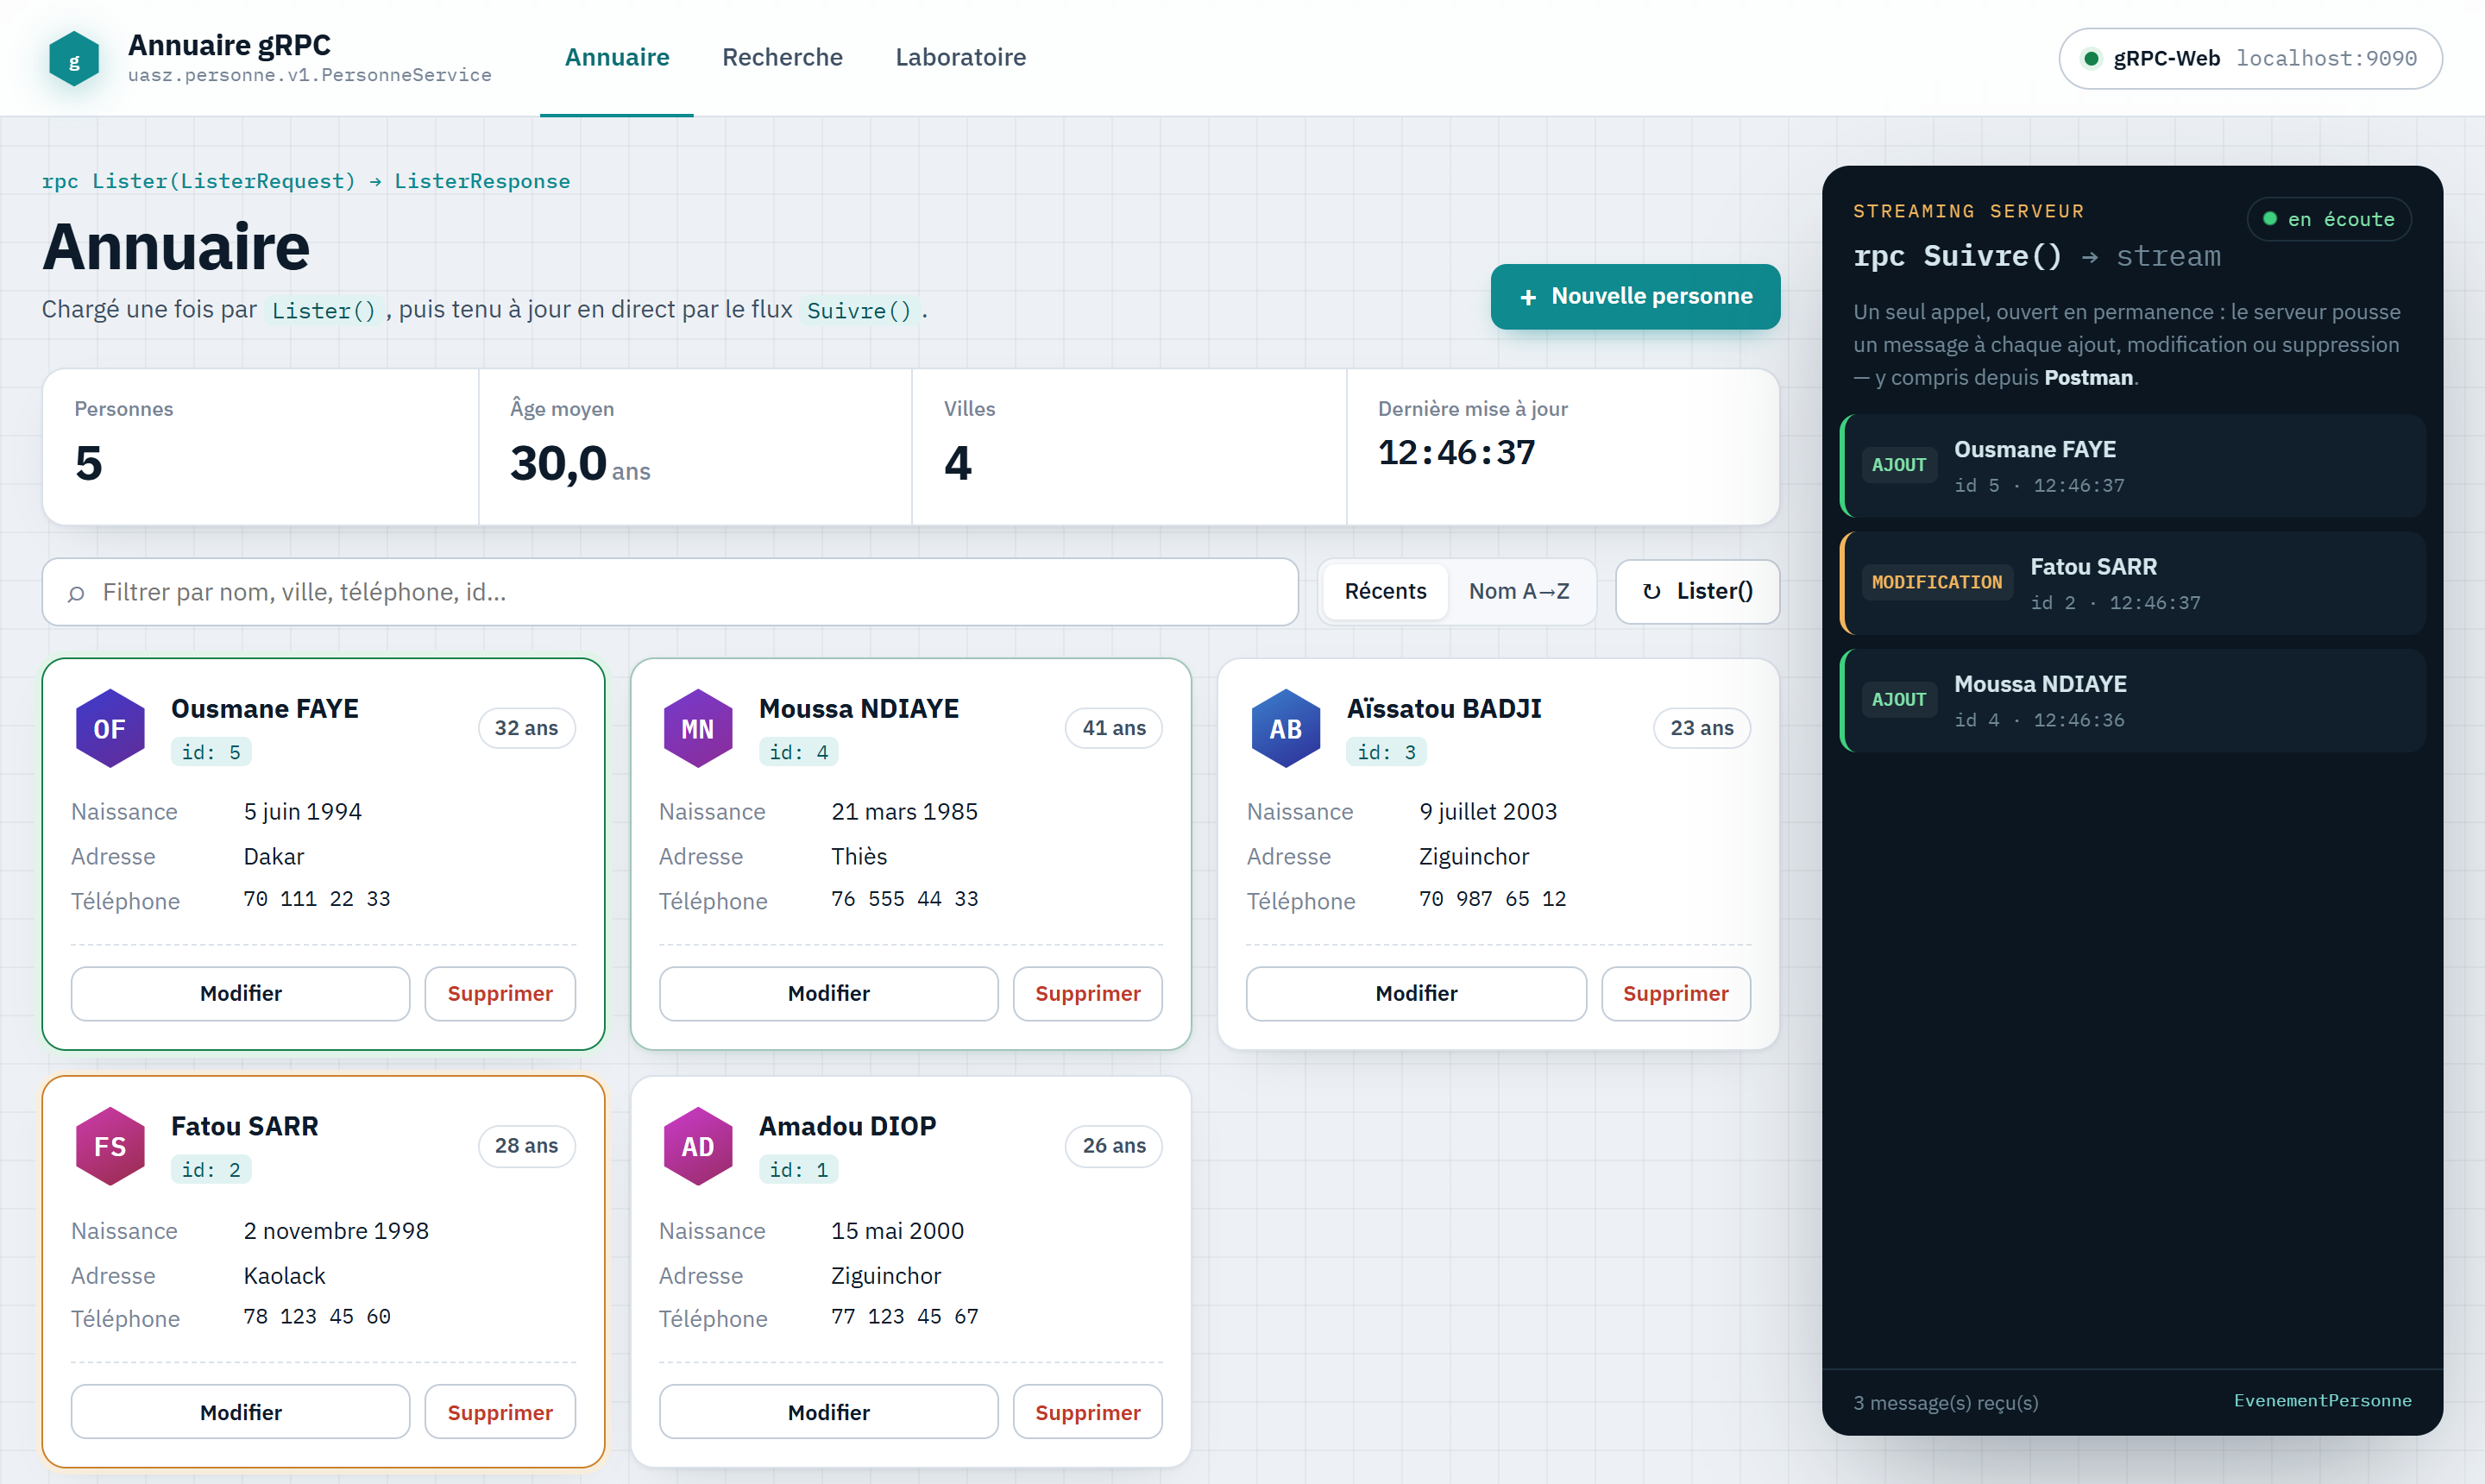
\includegraphics[height=5.45cm]{figures/annuaire.png}};
    \node[packet,anchor=west,visible on=<2->] at ([xshift=0.2cm,yshift=1.3cm]img.east) {flux Suivre()};
    \draw[flowback,visible on=<2->] ([xshift=0.2cm,yshift=1.3cm]img.east) -- ([xshift=-0.6cm,yshift=1.3cm]img.east);
    \node[tpacket,anchor=east,visible on=<3->] at ([xshift=-0.2cm,yshift=-0.7cm]img.west) {cartes};
    \draw[flow,visible on=<3->] ([xshift=-0.2cm,yshift=-0.7cm]img.west) -- ([xshift=0.5cm,yshift=-0.7cm]img.west);
  \end{tikzpicture}

  \vspace{0.05cm}
  \scriptsize Liste chargée par \mono{Lister()}, puis tenue à jour par \mono{Suivre()}~: vert = ajout, ambre = modification.
\end{frame}

\begin{frame}{Le laboratoire~: regarder « sur le fil »}
  \begin{columns}[c,onlytextwidth]
    \column{0.64\textwidth}
    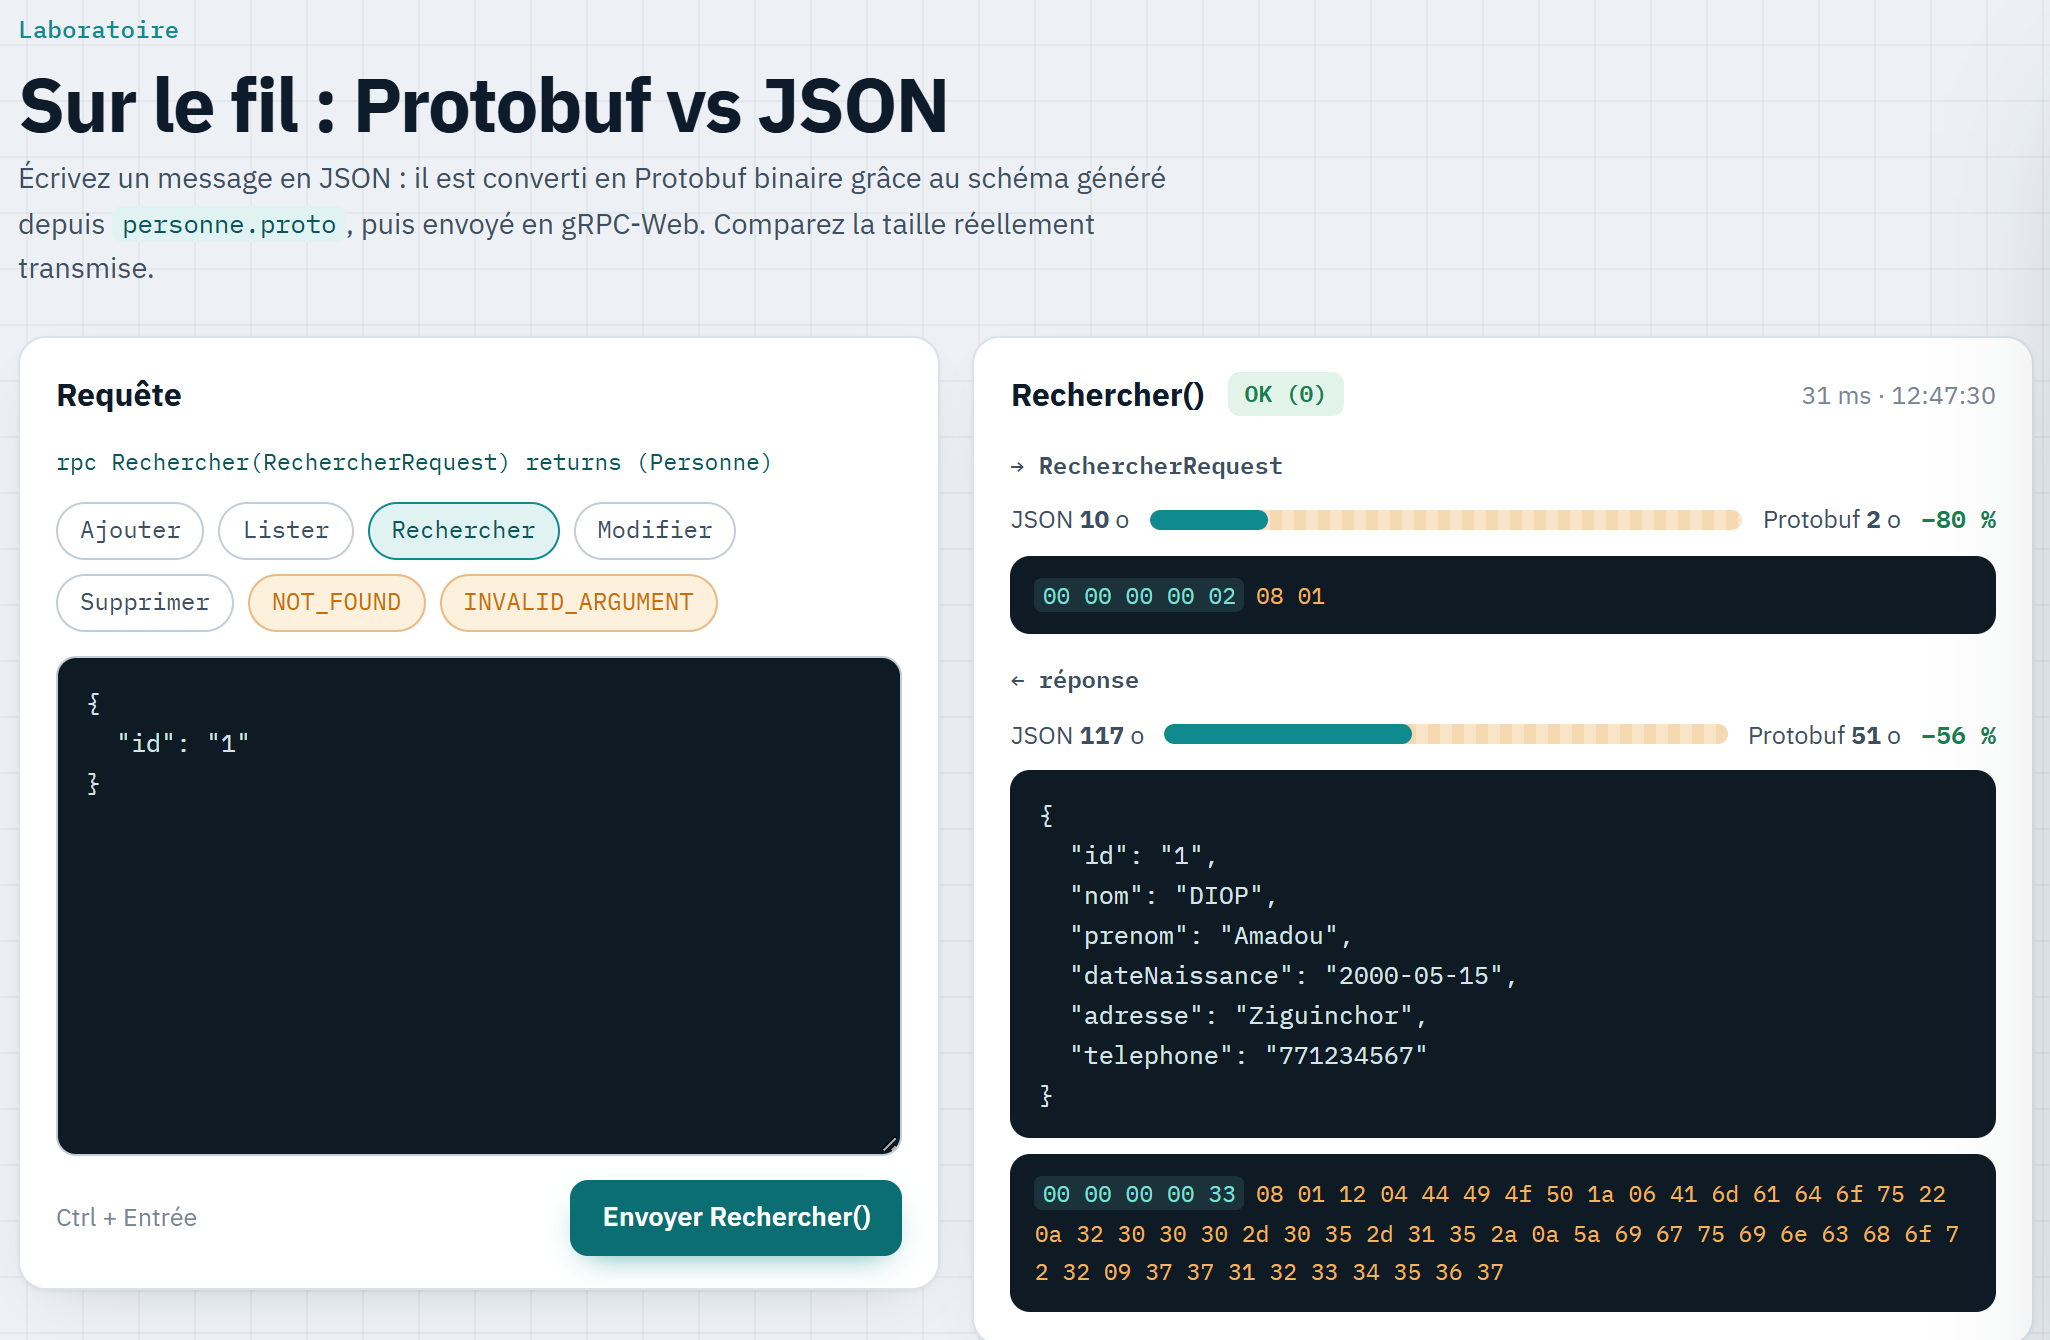
\includegraphics[width=\linewidth]{figures/laboratoire-zoom.png}
    \column{0.33\textwidth}\small
    \begin{itemize}
      \item On écrit le message en JSON
      \item Il est converti en \textbf{Protobuf} grâce au schéma généré
      \item On voit les \textbf{octets envoyés} et l'en-tête de trame
      \item Requête~: \textbf{2 octets} au lieu de 10~; réponse~: \textbf{51} au lieu de 117
    \end{itemize}
  \end{columns}
\end{frame}

\begin{frame}{Ajouter une personne, gérer une erreur}
  \begin{columns}[T,onlytextwidth]
    \column{0.52\textwidth}
    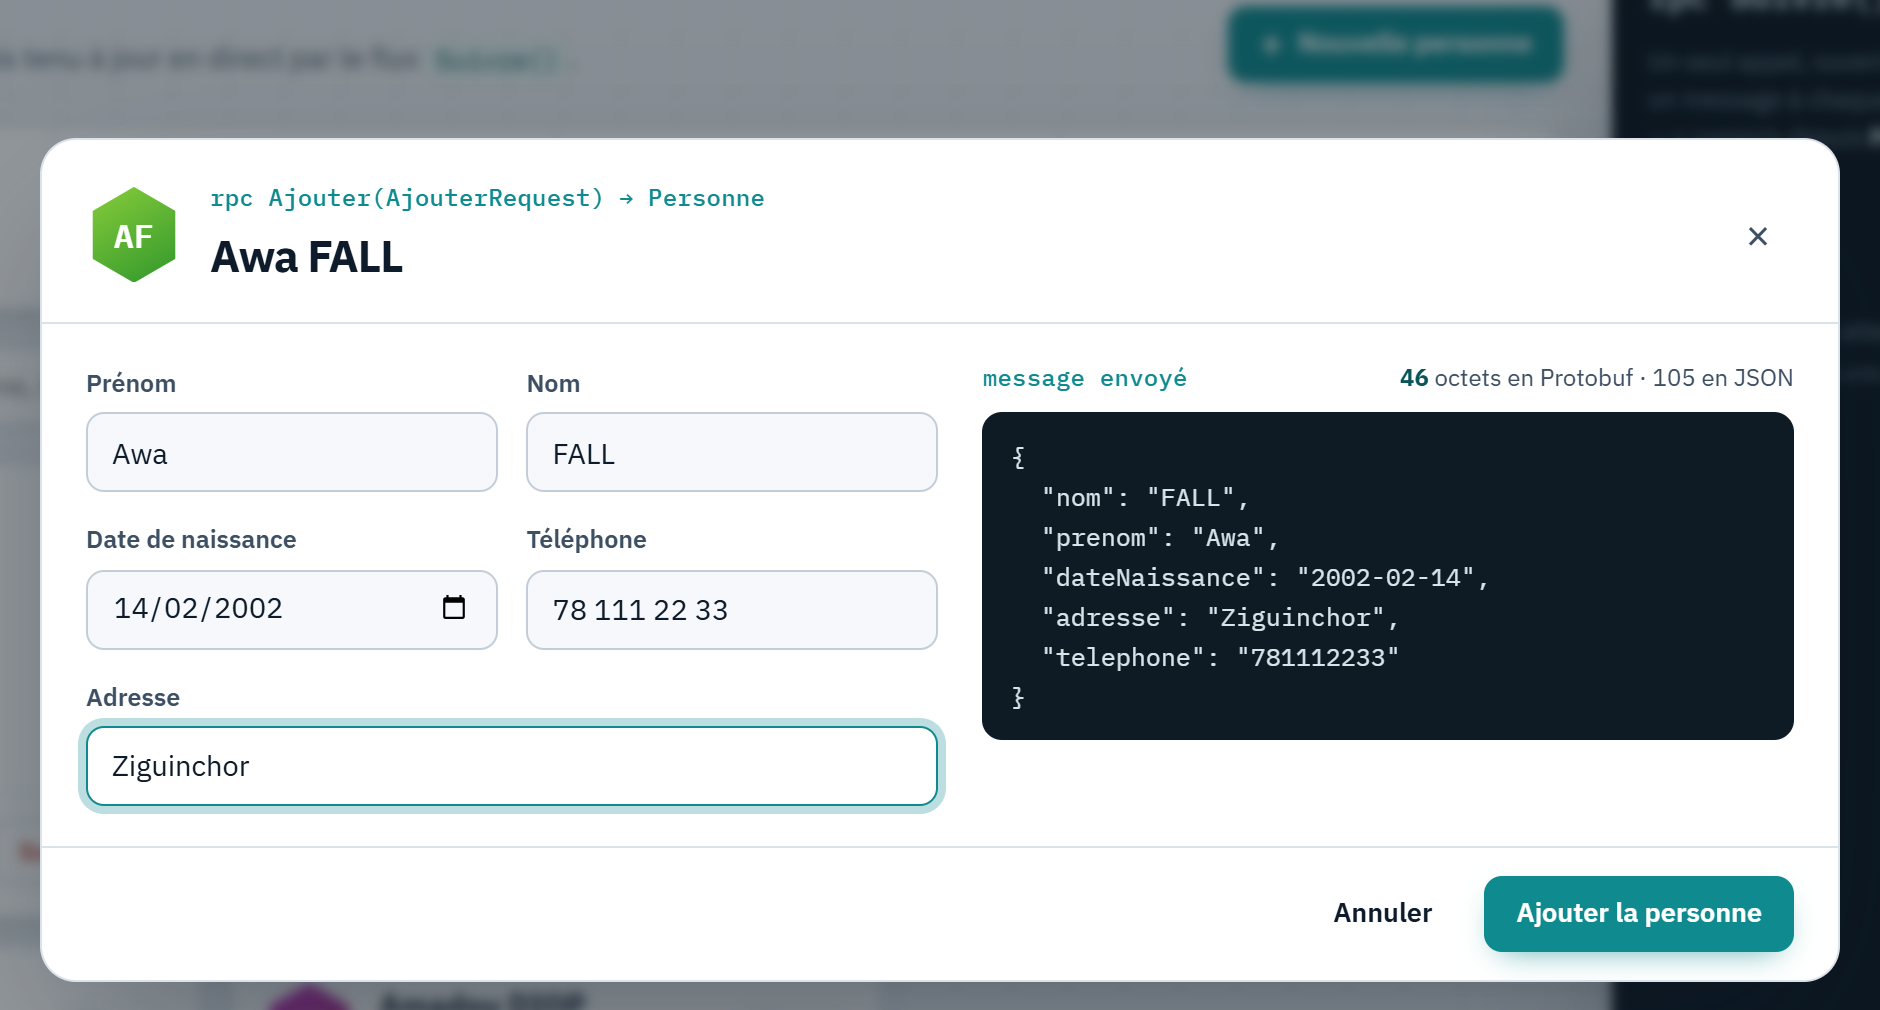
\includegraphics[width=\linewidth]{figures/dialogue-zoom.png}\par\vspace{3pt}
    {\scriptsize Le formulaire montre le message \mono{AjouterRequest} et sa taille~: 46 octets en Protobuf, 105 en JSON.}
    \column{0.45\textwidth}
    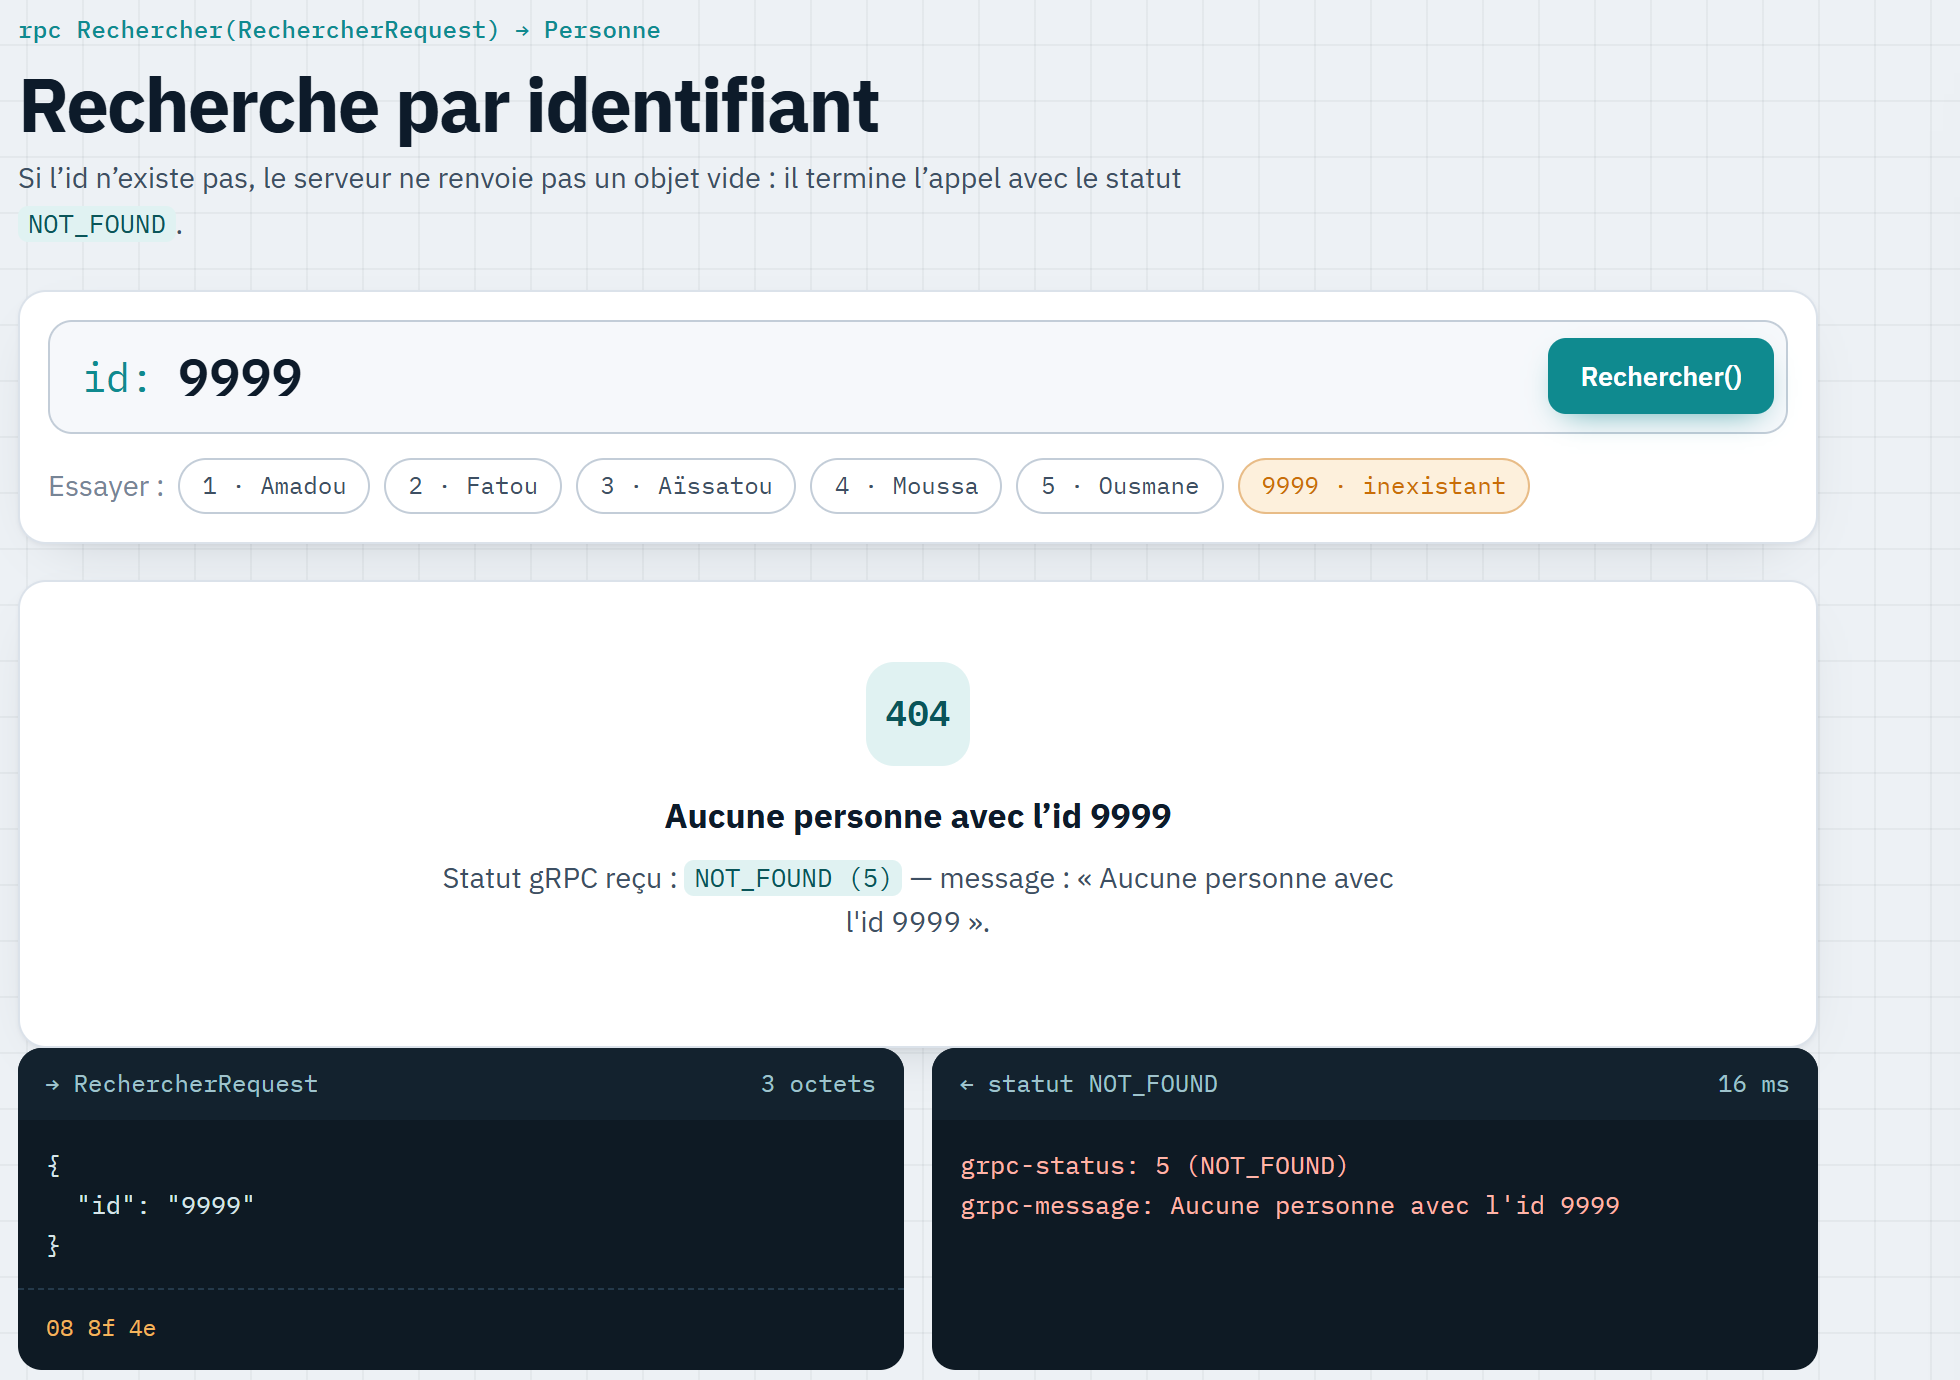
\includegraphics[width=\linewidth]{figures/not-found-zoom.png}\par\vspace{3pt}
    {\scriptsize \mono{Rechercher(\{id: 9999\})}~: le serveur termine l'appel avec \mono{NOT\_FOUND (5)}.}
  \end{columns}
\end{frame}

\begin{frame}{Déroulé de la démonstration}
  \centering
  \begin{tikzpicture}[x=1cm,y=1cm,
      etapebox/.style={box,minimum width=2.15cm,minimum height=2.0cm,text width=1.95cm,align=center,font=\scriptsize}]
    \foreach \i/\t/\d [count=\k from 0] in {
      1/Le contrat/{le \mono{.proto} et le code généré},
      2/Le serveur/{démarrage, tests, page \mono{/docs}},
      3/Postman/{réflexion, Ajouter, erreur},
      4/Angular/{annuaire, ajout, modification},
      5/Le flux/{Postman ajoute, le navigateur réagit},
      6/Sur le fil/{Protobuf contre JSON}} {
      \node[etapebox,visible on=<\i->] (s\i) at (\k*2.35,0) {\etape{\i}\\[3pt]{\bfseries\small\t}\\[2pt]{\color{Muted}\d}};
    }
    \foreach \a/\b in {1/2,2/3,3/4,4/5,5/6} \draw[flow,visible on=<\b->] (s\a) -- (s\b);
  \end{tikzpicture}

  \vspace{0.35cm}
  \uncover<6->{\begin{carte}[gteal]\small\faClock[regular]\enspace Environ 8 minutes. Tout se lance avec deux commandes~:
  \mono{mvnw spring-boot:run} (serveur) et \mono{npm start} (client).\end{carte}}
\end{frame}

\begin{frame}{À vous de jouer~: le TP gRPC}
  \begin{columns}[c,onlytextwidth]
    \column{0.66\textwidth}
    \begin{enumerate}\small
      \item Récupérer le dépôt et lancer le serveur (\mono{03-grpc/backend})
      \item Tester dans \textbf{Postman} les \textbf{5 méthodes} et \textbf{au moins 2 erreurs}
      \item Bonus~: \mono{Suivre}, \mono{Importer} et \mono{RechercherEnFlux}
      \item Écrire un \textbf{client dans une autre technologie} que Java~:
      \begin{itemize}\scriptsize
        \item navigateur (React, Vue, Svelte…)~: gRPC-Web sur \mono{localhost:9090}, CORS déjà ouvert
        \item Python (\mono{grpcio}), Node.js (\mono{@grpc/grpc-js}), Go, C\#…
      \end{itemize}
    \end{enumerate}
    \begin{carte}[gamber]\scriptsize\faBook\enspace Énoncé~: \mono{03-grpc/docs/TP\_gRPC.md}\\
    Contrat~: \mono{03-grpc/proto/personne.proto}\end{carte}
    \column{0.3\textwidth}
    \centering
    \begin{tcolorbox}[gcard,width=3.6cm,halign=center]
      \qrcode[height=2.7cm]{https://github.com/Massaly2609/web-services-uasz/tree/main/03-grpc}\par\vspace{3pt}
      {\tiny\ttfamily github.com/Massaly2609/\\web-services-uasz}
    \end{tcolorbox}
  \end{columns}
\end{frame}

% =====================================================================
\section{Conclusion}
% =====================================================================

\begin{frame}{À retenir}
  \vspace{0.1cm}
  \begin{columns}[T,onlytextwidth]
    \column{0.48\textwidth}
    \begin{carte}[gteal,height=2.15cm]\cartetitre{\etape{1}}{Un contrat d'abord}\footnotesize Le fichier \mono{.proto} décrit tout~; le code client et serveur est généré.\end{carte}
    \begin{carte}[gteal,height=2.15cm]\cartetitre{\etape{2}}{Rapide et compact}\footnotesize Protobuf binaire + HTTP/2~: des messages jusqu'à 10 fois plus petits dans nos mesures.\end{carte}
    \column{0.48\textwidth}
    \begin{carte}[gteal,height=2.15cm]\cartetitre{\etape{3}}{Le streaming natif}\footnotesize Quatre types d'appels, dont le flux serveur qui pousse les données en direct.\end{carte}
    \begin{carte}[gamber,height=2.15cm]\cartetitre{\etape{4}}{Le bon outil au bon endroit}\footnotesize Idéal entre microservices~; pour le navigateur, il faut gRPC-Web.\end{carte}
  \end{columns}
  \vspace{0.2cm}
  \centering\small XML-RPC (1998) → JSON-RPC → … → \textbf{gRPC}~: la même idée du RPC, \textbf{industrialisée}.
\end{frame}

\begin{frame}[plain,noframenumbering]
  \begin{tikzpicture}[remember picture,overlay]
    \fill[Navy] (current page.south west) rectangle (current page.north east);
    \draw[step=0.5cm,white,opacity=0.04] (current page.south west) grid (current page.north east);
    \node[hexa=2.3cm,fill=Teal] at ([xshift=-3.1cm,yshift=0.3cm]current page.center) {};
    \node[font=\ttfamily\bfseries\Huge,text=white] at ([xshift=-3.1cm,yshift=0.25cm]current page.center) {g};
    \node[anchor=west,text=white,font=\fontsize{34}{34}\selectfont\bfseries] at ([xshift=-1.5cm,yshift=0.65cm]current page.center) {Merci~!};
    \node[anchor=west,text=TealGlow,font=\Large] at ([xshift=-1.45cm,yshift=-0.35cm]current page.center) {Vos questions~?};
    \node[anchor=south,text=CodeMuted,font=\footnotesize] at ([yshift=0.8cm]current page.south) {Medoune MASSALY \enspace\&\enspace Alioune DIOUF \enspace\textperiodcentered\enspace Master 1 Web Services \enspace\textperiodcentered\enspace UASZ};
  \end{tikzpicture}
\end{frame}

\begin{frame}{Références}
  \small
  \begin{itemize}
    \item gRPC — documentation officielle~: \mono{grpc.io/docs}
    \item Protocol Buffers — guide du langage proto3~: \mono{protobuf.dev}
    \item Protocole gRPC sur HTTP/2~: \mono{github.com/grpc/grpc/blob/master/doc/PROTOCOL-HTTP2.md}
    \item gRPC-Web~: \mono{github.com/grpc/grpc-web} \enspace\textperiodcentered\enspace Connect-ES~: \mono{connectrpc.com}
    \item Codes de statut gRPC~: \mono{grpc.io/docs/guides/status-codes}
    \item HTTP/2~: RFC 9113 (2022, remplace la RFC 7540 de 2015)
    \item Armeria (serveur du TP)~: \mono{armeria.dev}
    \item I. Zhuang \& E. Anderson, \emph{gRPC in 5 minutes}, gRPC Day
    \item Cours de Web Services, Master 1, UASZ~: XML-RPC et JSON-RPC
  \end{itemize}
\end{frame}

\end{document}
